\documentclass{fast-nuces-bs}

\usepackage{blindtext}
\usepackage{mathptmx}% Times Roman font
\usepackage[T1]{fontenc}
\usepackage{lipsum} 
\usepackage{sectsty}
\usepackage{tikz-uml}
\usepackage{titlesec}

% Information about the Thesis 
% -----------------------------------------------------------------------------
% (All are compulsory, do not delete any line other than author Information)
% For e.g., usually there are 3 students in a group, so leave authorone, 
% authortwo, and authorthree, and delete authorfour.
%%%%%%%%%%%%%%%%%%%%%%%%%%%%%%%%%%%%%%%%%%%%%%%%%%%%%%%%%%%%%%%%%%%%%%%%%%%%%%%
\department{Department of Computer Science}
\faculty{Computer Science}
\degreeyear{2025}
\degreemonth{June}
\degreename{Computer Science}
\campuscity{Peshawar}
\authorone{Muhammad Ayan Shabbir}{21P-8035}
\authortwo{Abdus Samad Kaleem}{21P-8011}
\authorthree{Sher Ali}{21P-8024}
\supervisor{Dr. Muhammad Amin}
\sessionduration{2021-2025}
% \cosupervisor{Mr./ Ms./ Dr. Supervisor Name}
% \deanname{Dr. Dean Computing}
\directorname{Dr. Omar Usman}
\hodname{Mr. Fazl e Basit}
\fypcoordinatorname{Mr. Haroon Zafar}
\title{HiringGuru: AI Career Assistance & Real-Time
Interview Feedback}
%%%%%%%%%%%%%%%%%%%%%%%%%%%%%%%%%%%%%%%%%%%%%%%%%%%%%%%%%%%%%%%%%%%%%%%%%%%%%%%

%%%%%%%%%%%%%%%%%%%%%%%%%%%%%%%%%%%%%%%%%%%%%%%%%%%%%%%%%%%%%%%%%%%%%%%%%%%%%%
% Former document starts below this
\begin{document}

\begin{acknowledgements}
	Your acknowledgments here
\end{acknowledgements}

\begin{abstract}
The research addresses the problem of limited tools for effective interview preparation, particularly in providing personalized feedback on non-verbal cues like posture and facial expressions. Job candidates often struggle to gauge their performance in terms of both content and demeanor, a challenge that standard mock interview platforms do not fully address. This project introduces an AI-driven application designed to simulate real-world interview conditions, capturing and analyzing users’ facial expressions, posture, and responses in real-time. The application utilizes deep learning techniques for posture detection and natural language processing to assess user answers. The methodology includes implementing machine learning models for expression and posture recognition, paired with a feedback algorithm to generate an in-depth performance report.

Key results demonstrate that users gain improved self-awareness in interview scenarios, with early testing showing a measurable boost in posture awareness and response confidence. However, limitations in real-time processing under certain network conditions were identified. In conclusion, this AI-powered interview simulator provides a novel approach to interview practice, enhancing both verbal and non-verbal skills through targeted feedback. Further improvements in processing efficiency and customization could expand its applicability across various professional fields.
\end{abstract}

\chapter{Introduction} \label{sec
}

\section{Purpose of the Investigation}

The purpose of this investigation is to design and develop an AI-powered application that enables users to practice and enhance their interview skills. By creating a simulated interview environment, this application aims to assess key aspects of a candidate’s performance—such as body language, facial expressions, and verbal responses—through real-time analysis. The tool seeks to provide job seekers with meaningful feedback, helping them to better prepare for actual interview situations and improve their overall employability.

\section{Problem Being Investigated}

Despite the availability of abundant career guidance resources, candidates often struggle to gain insights into the quality of their interview skills. Traditional interview preparation methods lack interactive feedback on posture, facial expressions, and response delivery, which are critical components of a successful interview. The absence of such personalized and interactive feedback can hinder candidates’ ability to refine their presentation, leading to suboptimal interview performances. This investigation addresses the need for an advanced tool that uses AI to close this gap in interview preparation.

\section{Background and Importance of the Problem}

Interview preparation has evolved with advancements in technology, but many existing solutions are limited to static resources or basic question-and-answer formats. Previous research has demonstrated the effectiveness of feedback in improving interview skills, but few tools provide real-time analysis. By leveraging AI, facial recognition, and body language detection, this project builds on previous efforts to offer a more dynamic and personalized experience. Studies have shown that such technologies can significantly impact confidence and presentation in job interviews, underlining the importance of this application \cite{test}.

\section{Thesis and General Approach}

This thesis proposes that an AI-driven, interactive interview practice platform can improve job candidates' readiness by providing actionable feedback on their performance. The approach involves using computer vision and natural language processing to evaluate non-verbal cues, such as facial expressions and posture, and verbal responses to simulated interview questions. The platform will conclude each session with a comprehensive report detailing areas for improvement, effectively bridging the gap between theoretical preparation and practical application.

\section{Criteria for Study’s Success}

The success of this study will be determined by the following criteria:

\begin{itemize} \item Accuracy: The AI should accurately analyze facial expressions, posture, and verbal responses during interviews. \item Usability: The application should be user-friendly, making it accessible to a wide range of users with minimal technical expertise. \item Effectiveness: Feedback provided by the application should enable users to enhance their interview skills meaningfully. \item Engagement: The platform should simulate a realistic interview experience to engage users and increase preparation quality. \item Reliability: The tool should deliver consistent results across different sessions and scenarios. \end{itemize}
\chapter{Review of Literature} \label{ch
}

The literature review explores recent advancements in AI-powered interview platforms, pose and posture recognition, and real-time feedback mechanisms. This section provides a critical overview of state-of-the-art technologies in these areas, examining their methodologies, findings, and limitations. By synthesizing this information, this review identifies gaps in existing research and highlights the potential for further development in AI-driven interview preparation tools.

\section{Introduction} The purpose of this literature review is to establish a foundation for developing an AI-powered interview practice application that enhances interview readiness through real-time feedback on expressions, posture, and response quality. This review focuses on recent studies (within the last five years) that have explored interview simulations, pose detection technologies, and interactive feedback systems, aiming to provide insights into their contributions and limitations.

\section{Body} Each source is summarized and critically evaluated based on its research design, methodologies, and findings. The following section presents key studies relevant to this project, focusing on their approaches, contributions to interview preparation, and any identified gaps in technology or application.

\subsection{Tabular Analysis of Literature} The table below provides an organized summary of the reviewed literature, highlighting essential aspects such as methodologies, results, and limitations.

\begin{table}[h]
\centering
\begin{tabular}{|c|c|p{3.5cm}|p{3.5cm}|p{2.5cm}|p{3.5cm}|}
\hline
\textbf{Ref. No} & \textbf{Year} & \textbf{Basic Idea} & \textbf{Methodologies} & \textbf{Results} & \textbf{Limitations} \\ \hline
\cite{test} & 2024 & Mock interview platform with feedback & AI-powered interviews, personalized feedback & Improved interview skills & Not real-time monitoring, no posture correction \\ \hline
[2] & 2024 & Pose recognition technology (Viso.ai) & Deep learning & Accurate pose estimation for various applications & Detects only laying down, sitting, standing; no angle detection \\ \hline
[3] & 2024 & Interview warm-up platform & AI-powered practice questions, answer analysis & Increased confidence, interview preparedness & Only transcribes answers \\ \hline
[4] & 2023 & Hybrid posture detection framework & Machine learning, deep neural networks & Improved posture detection accuracy & High computational needs, data requirements, overfitting risk, real-time delays \\ \hline
[5] & 2022 & EZInterviewer, AI-driven tool for mock interviews & Natural language processing, machine learning & Personalized feedback, real-world simulation & Limited question variety, potential bias; no posture, facial detection \\ \hline
[6] & 2017 & Face detection, posture recognition for tracking systems & Machine learning (CNNs, keypoint detection) & Enhanced accuracy, efficiency in real-time face detection & Sensitive to lighting, occlusion issues, high computational demands, privacy concerns \\ \hline
\end{tabular}
\caption{Tabular Analysis of Reviewed Literature}
\label{tab:lit-review}
\end{table}


\section{Conclusion} The review of literature reveals that while there has been considerable progress in AI-powered interview and posture detection platforms, existing solutions often lack real-time monitoring, comprehensive posture correction, or a holistic assessment of interview skills. Notably, there is a gap in applications that combine posture analysis, facial expression tracking, and detailed response feedback in a single platform. These findings underscore the need for an integrated system capable of providing job seekers with a thorough, AI-driven assessment of their interview readiness. This project seeks to address these gaps by developing a comprehensive, real-time interview practice tool, informed by the insights gathered from existing research.



\chapter{Project Vision} \label{ch
}

This chapter provides an overview of the project's purpose, objectives, and anticipated impact. It discusses the problem the project aims to address, the business opportunities associated with it, and the project's scope, constraints, and stakeholders.

\section{Problem Statement} The current job market is highly competitive, with job seekers needing advanced skills and confidence to excel in interviews. Traditional interview preparation methods often lack personalized feedback on key elements like posture, facial expressions, and response quality. This project addresses the need for an interactive, AI-driven tool that provides real-time feedback on these aspects, empowering candidates to enhance their interview skills and improve their chances of success.

\section{Business Opportunity} There is a growing demand for professional development tools that leverage AI to enhance job seekers' readiness. This project presents an opportunity to capitalize on this trend by developing a platform that can be marketed to career development firms, educational institutions, and individuals seeking to improve their interview skills. The application's unique focus on real-time feedback for posture, expressions, and verbal responses distinguishes it from other interview preparation tools, creating a competitive advantage in the market.

\section{Objectives} The primary objectives of this project are as follows: \begin{itemize} \item Develop an AI-powered platform that enables users to practice interviews in a realistic, interactive environment. \item Provide real-time analysis of users' facial expressions, posture, and verbal responses. \item Generate comprehensive feedback reports to guide users in improving their interview skills. \item Ensure that the platform is user-friendly, accessible, and capable of delivering accurate, reliable feedback. \end{itemize}

\section{Project Scope} The project scope includes designing, developing, and deploying an AI-based interview practice platform with the following core features: \begin{itemize} \item Integration of webcam-based tracking to analyze facial expressions and body posture. \item An interactive interview simulation that asks users relevant questions based on their chosen field. \item Real-time feedback on user performance, focusing on non-verbal cues and response quality. \item A final report that highlights strengths, areas for improvement, and specific suggestions for enhancement. \end{itemize}

Features outside the current scope include advanced language processing beyond basic answer analysis, integration with external job platforms, and the ability to handle group interviews.

\section{Constraints} The project faces several constraints, including: \begin{itemize} \item Technical Constraints: Limitations in AI accuracy for facial and posture recognition in varied lighting or occluded environments. \item Computational Requirements: The need for high computational power for real-time processing, which may impact performance on lower-end devices. \item Privacy Concerns: Ensuring user data security and privacy during the collection, analysis, and storage of video data. \item Resource Limitations: Limited access to diverse datasets for training the AI models, which could impact the robustness of the feedback. \end{itemize}

\section{Stakeholders Description} The project involves various stakeholders, each with specific interests and goals associated with the application.

\subsection{Stakeholders Summary} The key stakeholders include: \begin{itemize} \item End Users: Job seekers who want to improve their interview skills. \item Educational Institutions: Universities and career development centers that can use the platform as a training tool. \item Career Development Firms: Organizations specializing in helping clients prepare for interviews. \item Development Team: Responsible for designing, developing, and maintaining the application. \end{itemize}

\subsection{Key High-Level Goals and Problems of Stakeholders} \begin{itemize} \item End Users: Seek a reliable, easy-to-use tool that offers actionable feedback for improving interview performance. They may face challenges in finding personalized guidance in conventional interview preparation resources. \item Educational Institutions: Aim to provide students with advanced resources to prepare for the job market, focusing on accessibility and integration with existing curricula. \item Career Development Firms: Interested in providing clients with the latest AI tools to gain an edge in the job market, but may have concerns about data privacy and accuracy of feedback. \item Development Team: Aims to build a robust, scalable, and user-friendly platform, with potential challenges related to technical feasibility, data handling, and resource management. \end{itemize}


\chapter{Software Requirements Specifications} \label{ch
}

This chapter outlines the detailed functional and non-functional requirements for the project. It includes descriptions of the main features, quality attributes, and system specifications to guide the development process.

\section{List of Features} The primary features of the project include: \begin{itemize} \item Real-time posture and facial expression analysis using AI. \item Interactive interview simulation with dynamic question selection. \item Detailed feedback and analysis report on user performance. \item User account management, including login, signup, and profile settings. \item Integration with webcam for real-time feedback. \end{itemize}

\section{Functional Requirements} The functional requirements detail the specific functions and capabilities of the system: \begin{itemize} \item The system shall allow users to log in, sign up, and manage their profiles. \item The system shall analyze users' facial expressions and posture through the webcam. \item The system shall present users with interview questions and evaluate their responses. \item The system shall generate a feedback report, highlighting performance and improvement areas. \item The system shall support both manual and Google login options. \end{itemize}

\section{Quality Attributes} Quality attributes are non-functional characteristics that are crucial for system success: \begin{itemize} \item Usability: The system should provide an intuitive and easy-to-use interface. \item Reliability: The feedback provided by the AI should be accurate and dependable. \item Performance: The system should perform real-time analysis without noticeable delays. \item Scalability: The platform should handle a high number of users with minimal performance degradation. \item Security: All user data, including video data, must be securely handled and stored. \end{itemize}

\section{Non-Functional Requirements} Non-functional requirements define system characteristics: \begin{itemize} \item Performance Requirements: The analysis of user performance should complete within 2 seconds of response. \item Security Requirements: User data should be encrypted and securely stored. \item Accessibility: The application should be accessible to people with different levels of computer proficiency. \item Compatibility: The application should be compatible with standard webcam devices and browsers. \end{itemize}

\section{Use Cases/ Use Case Diagram} The use case diagram in Figure~\ref{fig
} below illustrates the system’s interactions with different types of users. It highlights how various actors engage with key system functionalities, providing a high-level view of user roles and their access to features.

\begin{figure}[h] \centering 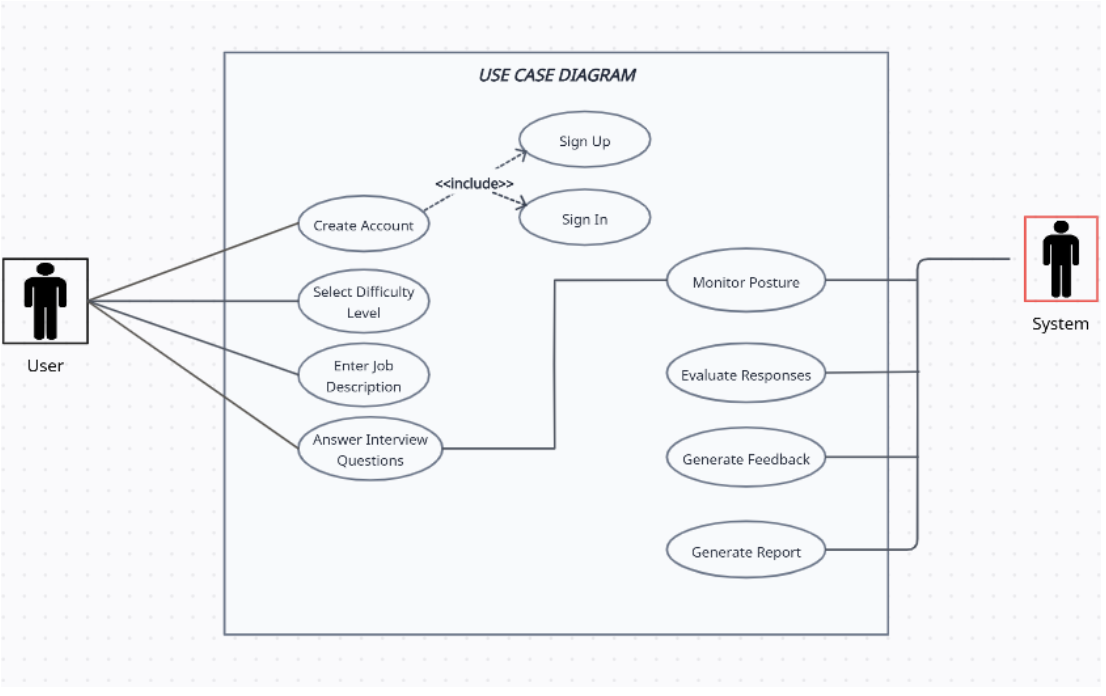
\includegraphics[width=0.5\linewidth]{sections/diagrams/UseCase.png} \caption{Use Case Diagram of the System} \label{fig
} \end{figure}

\section{Sequence Diagrams/System Sequence Diagram} This section includes sequence diagrams that illustrate the order of interactions within the system. These diagrams depict the step-by-step processes for key functionalities, such as user login, interview simulation, and report generation. They provide a clear visualization of how users interact with the system and how various components communicate to execute tasks efficiently.

\begin{figure}[h] \centering 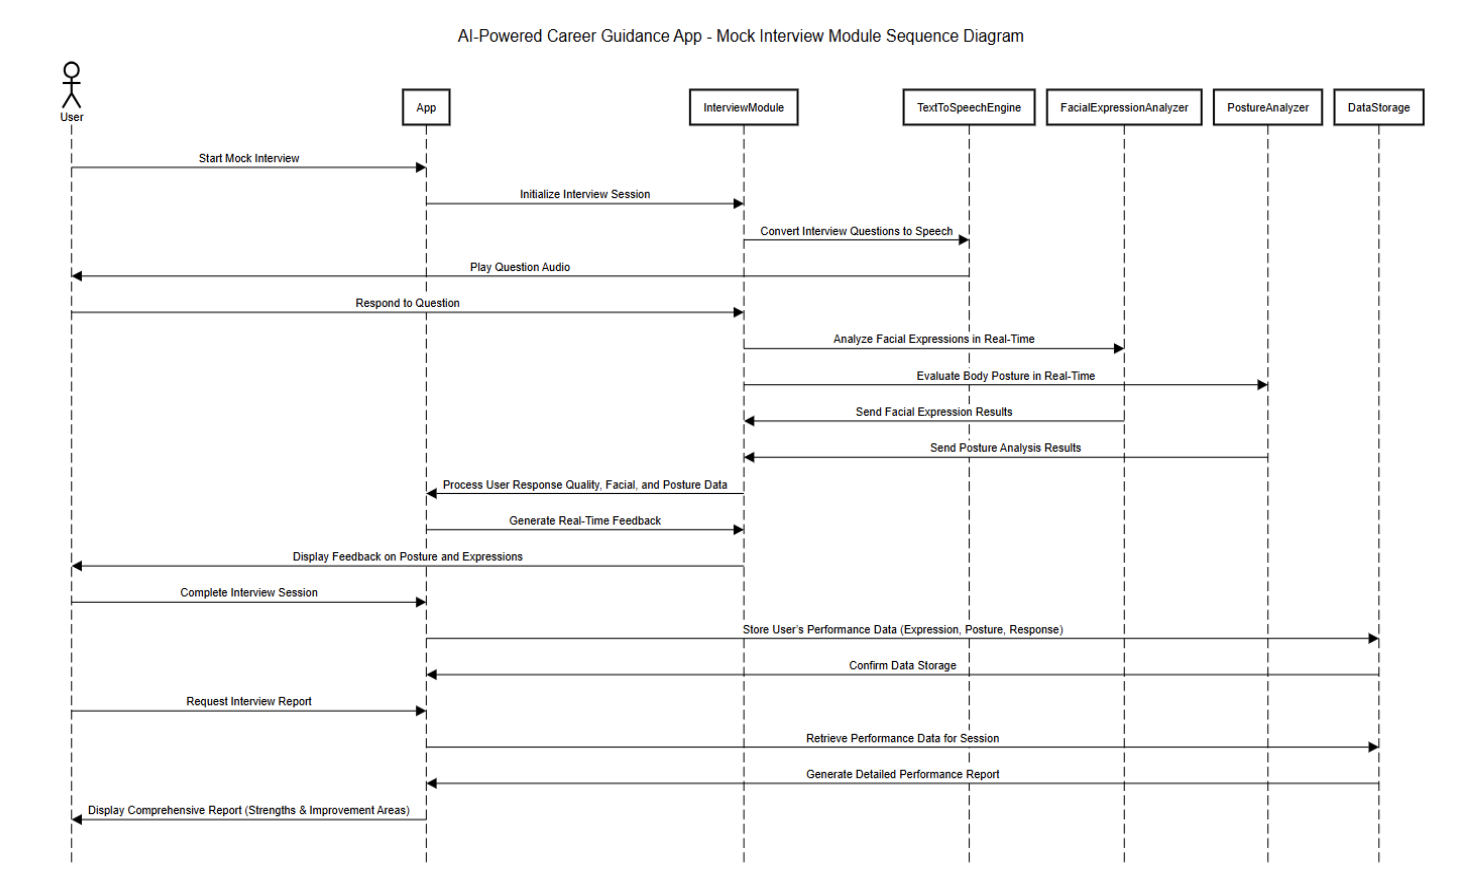
\includegraphics[width=0.5\linewidth]{sections/diagrams/SequentialModel.png} \caption{Sequence Diagram of Key Functionalities} \label{fig
} \end{figure}

\section{Architecture Diagram} This section includes an architecture diagram that illustrates the overall structure of the system. The diagram provides a high-level view of the system's components and their interactions, highlighting how different modules communicate with each other. Key functionalities such as user login, interview simulation, and report generation are represented, showcasing the integration of various technologies and frameworks that support the application’s operation.

\begin{figure}[h] \centering 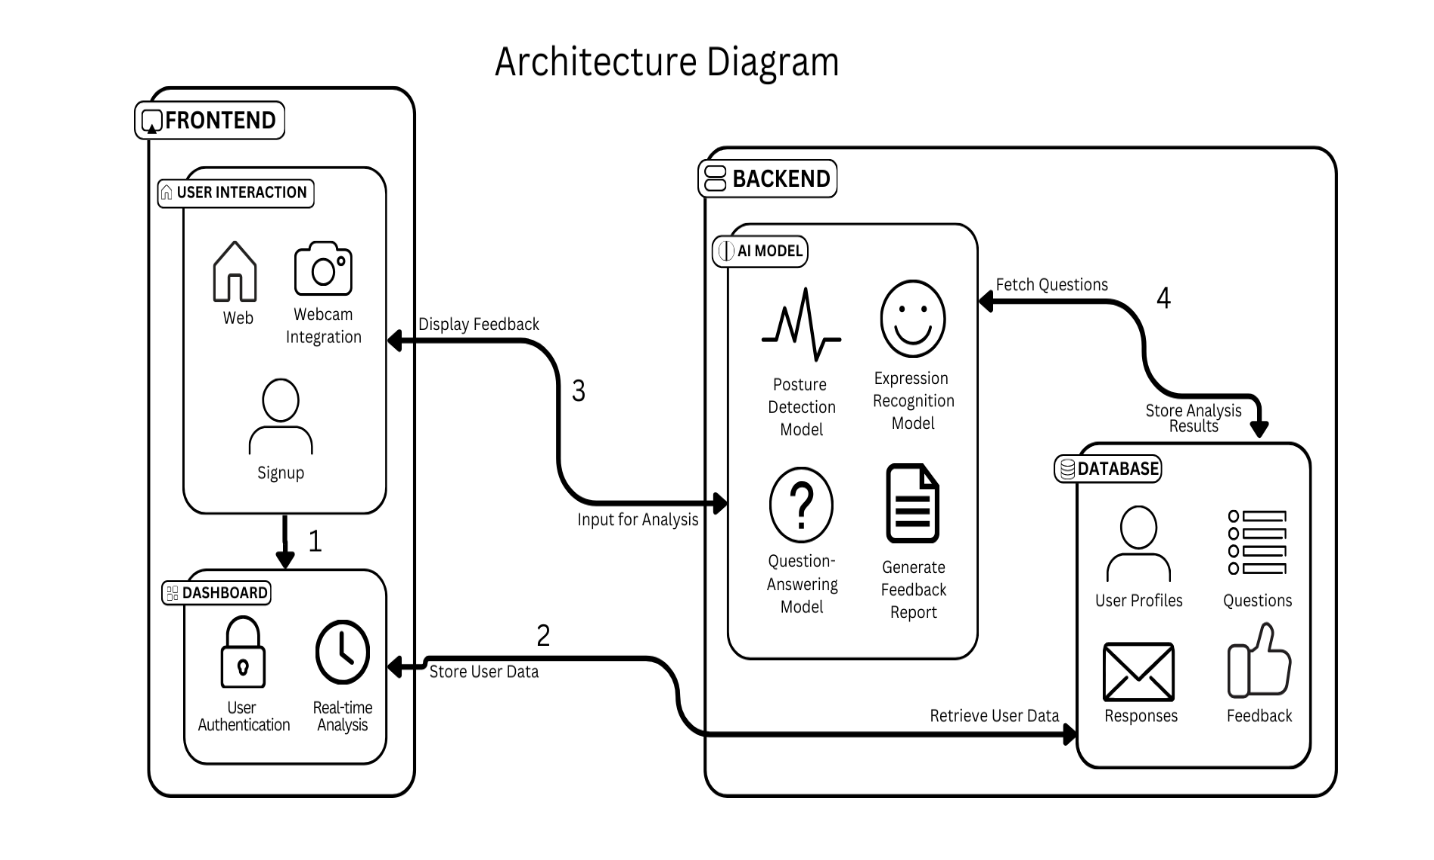
\includegraphics[width=0.5\linewidth]{sections/diagrams/ArchitectureDiagram.png} \caption{Architecture Diagram of the System} \label{fig
} \end{figure}

\section{Test Plan (Test Level, Testing Techniques)} The test plan will outline the levels of testing, including: \begin{itemize} \item Unit Testing: Testing individual components, such as user authentication and report generation. \item Integration Testing: Ensuring all system components work together, including the AI analysis and report generation. \item System Testing: Testing the complete system functionality and performance under various conditions. \item User Acceptance Testing (UAT): Ensuring the final product meets user expectations and requirements. \end{itemize}

Testing techniques will include both manual and automated testing.

\section{Software Development Plan} The software development plan will detail the project timeline, development methodology (e.g., Agile), key milestones, and resource allocation. Development phases will cover requirements gathering, design, implementation, testing, and deployment.

\section{Wire-frames} This section will include wireframes of the major screens in the application, such as the login page, interview simulation screen, and feedback report page. Wireframes provide a visual blueprint for the user interface and layout.

\section{UI Screens} The UI screens will include final designs of the user interface, showcasing elements like buttons, navigation, and layout for a consistent user experience. These will be developed based on the wireframes and refined to ensure usability and visual appeal.
\chapter{Iteration Plan}
\label{ch:iter0}

This chapter describes the iteration plan for the project, outlining how the development progresses to meet all requirements. It provides an overview of the project modules and their phased development. The execution of the project is divided into the following phases:

\begin{itemize}
    \item Midterm FYP 1
    \item Final FYP 1
    \item Midterm FYP 2
    \item Final FYP 2
\end{itemize}

\section{Midterm FYP 1}
During the Midterm of FYP 1, the primary focus was on data collection for posture detection and interview Q/A analysis. Additionally, a pre-trained model for facial expression recognition was explored and selected. The initial frontend setup and UI design were also completed in this phase, laying the foundation for further development.

\section{Final FYP 1}
By the Final FYP 1, the collected data was preprocessed for posture detection, ensuring its quality for training purposes. The pre-trained facial expression model was successfully integrated into the system. Furthermore, basic UI functionalities were developed, providing an interface for user interaction with the system.

\section{Midterm FYP 2}
The Midterm of FYP 2 focused on training the posture detection model using a hybrid approach combining MobileNetV2 and MediaPipe. The facial expression model was tested and validated to ensure its performance met the required standards. Additionally, backend development was initiated, along with API integration, enabling smooth data flow between different components.

\section{Final FYP 2}
In the Final FYP 2, the full system integration was completed, bringing together posture detection, facial expression analysis, and interview Q/A processing. Performance tuning and evaluation were carried out to enhance accuracy and efficiency. Finally, rigorous testing was conducted before deployment, ensuring that the system met all the necessary requirements.

% \begin{figure}[h] \centering 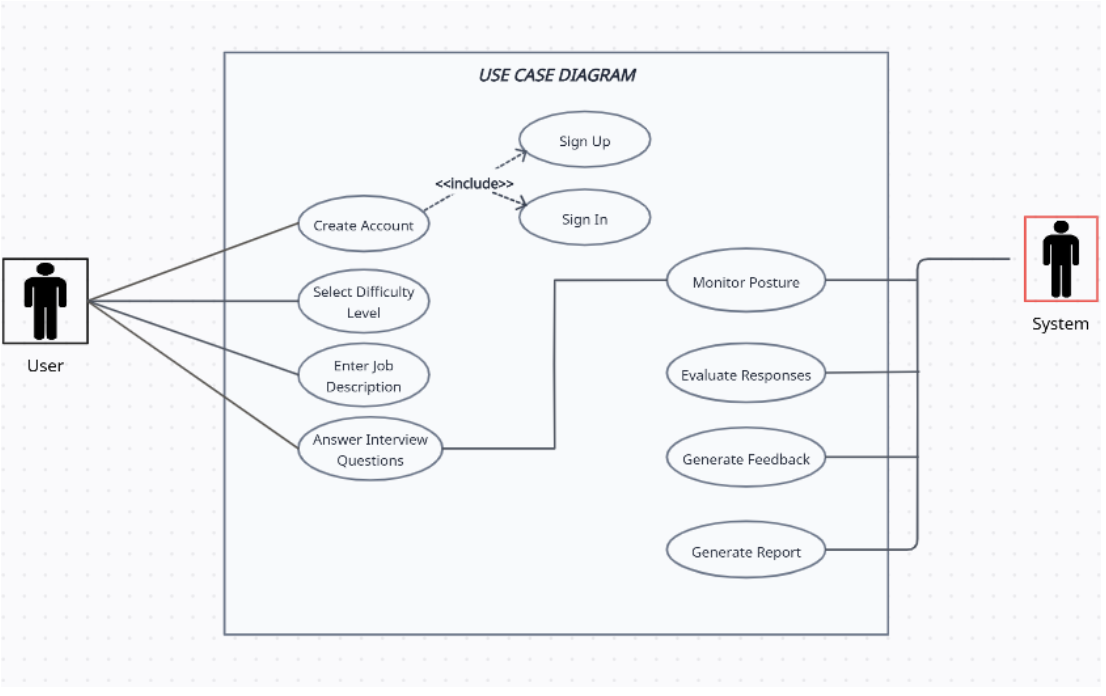
\includegraphics[width=0.5\linewidth]{sections/diagrams/UseCase.png} \caption{Use Case Diagram of the System} \label{fig
% } \end{figure}
\chapter{Iteration 1}
\label{ch:iter1}

The first iteration of the project, \textbf{HiringGuru – A Real-Time AI Mock Interview System}, is designed to be completed by the midterm evaluation of FYP-1. This chapter elaborates on the system design, development practices, and testing strategies implemented in this iteration. The design is categorized into structural and behavioral components, followed by detailed development, maintainability, and system-level artifacts.

\section{Structural Design}

\subsection{Domain Model / Class Diagram}
The domain model identifies key entities such as \texttt{User}, \texttt{InterviewSession}, \texttt{AnalysisModule}, and \texttt{DatabaseHandler}. These classes interact to perform core functionalities including posture detection, facial expression analysis, question generation, and result recording, forming the backbone of HiringGuru.

\subsection{Component Diagram}
The system comprises multiple decoupled components. The frontend is built with \textbf{Next.js}, while the backend uses \textbf{Node.js}. It integrates with the \textbf{OpenAI API} for dynamic question generation, \textbf{TensorFlow} and \textbf{OpenCV} for real-time video analysis, and \textbf{Firebase} for database operations and authentication.

\subsection{Layered Architecture}
HiringGuru follows a standard three-tiered architecture:

\begin{itemize}
  \item \textbf{Presentation Layer:} Developed using Next.js and styled with TailwindCSS.
  \item \textbf{Business Logic Layer:} Handles AI analysis logic, including posture detection (MobileNetV2 + MediaPipe) and facial expression recognition (Haarcascade + Dlib).
  \item \textbf{Data Layer:} Firebase is used to store user profiles, session data, and analysis results securely.
\end{itemize}

\subsection{Structure Chart}
The structure chart illustrates function-level decomposition, outlining modules such as:
\begin{itemize}
  \item Posture Analysis (\texttt{MobileNetV2 + MediaPipe})
  \item Facial Expression Recognition (\texttt{Haarcascade + Dlib})
  \item Question-Answer Processing (\texttt{OpenAI API})
\end{itemize}

\section{Behavioral Design}

\subsection{Flow Diagram}
The interaction flow is summarized as follows:
\begin{enumerate}
  \item The user logs in and initiates a mock interview session.
  \item The webcam starts capturing real-time video.
  \item AI modules analyze posture and facial expressions.
  \item Interview questions are generated using OpenAI API.
  \item User responses are analyzed and stored.
\end{enumerate}

\subsection{Data Flow Diagram (DFD)}
The DFD represents the movement of data through the system—from the video input captured via webcam to processing with TensorFlow/OpenCV, and finally to Firebase for persistent storage. User responses are also transmitted back to the frontend for immediate feedback.

\subsection{Data Dictionary}
The key data entities and their attributes include:

\begin{itemize}
  \item \textbf{User:} \texttt{UserID}, \texttt{Name}, \texttt{Email}, \texttt{Role}
  \item \textbf{Interview Session:} \texttt{SessionID}, \texttt{Timestamp}, \texttt{Questions}, \texttt{Responses}
  \item \textbf{Analysis Data:} \texttt{PostureScore}, \texttt{FacialExpression}, \texttt{Accuracy}
\end{itemize}

\subsection{Activity Diagram}
The activity diagram illustrates the flow from initializing the interview session to capturing frames, performing AI-based analysis, and displaying feedback. It captures the continuous loop until the session ends.

\subsection{State Machine Diagram}
The system’s operational states are defined as:

\begin{itemize}
  \item \textbf{Idle:} Waiting for user interaction.
  \item \textbf{Analyzing:} Capturing and processing video.
  \item \textbf{Responding:} User replies to questions.
  \item \textbf{Evaluating:} AI evaluates user response and expressions.
  \item \textbf{Completed:} Interview ends, results are compiled.
\end{itemize}

\subsection{Sequence Diagram}
The sequence diagram traces communication between frontend, backend, AI models, and external APIs. It captures call sequences for video processing, real-time data transmission, and OpenAI interaction.

\subsection{Interaction Overview Diagram}
This hybrid diagram integrates sequence and activity views, emphasizing the major system interactions as users proceed through the mock interview lifecycle.

\section{Schema Design / ER Diagram}
The Entity-Relationship (ER) diagram models the underlying database structure, comprising entities such as \texttt{User}, \texttt{InterviewSession}, \texttt{AIQuestionBank}, \texttt{AnalysisData}, and \texttt{Logs}. Relationships among these entities are defined to ensure normalized and scalable storage.

\section{Data Structure Design}
Optimized data structures, including multidimensional arrays, hash maps, and tensors, are employed to handle high-throughput video frames and low-latency AI analysis for real-time processing.

\section{Algorithm Design}
Core algorithms and frameworks integrated into the system include:

\begin{itemize}
  \item \textbf{MobileNetV2 + MediaPipe:} For accurate, lightweight posture detection with $\sim$90\% accuracy.
  \item \textbf{Haarcascade + Dlib:} For robust facial expression detection.
  \item \textbf{TensorFlow:} Powers custom-trained models for performance scoring and emotion classification.
  \item \textbf{OpenAI API:} Generates context-aware, adaptive interview questions.
\end{itemize}

\section{Development Phase}

\subsection{Comments, Naming Conventions, and Static Analysis}
All modules follow consistent and descriptive naming conventions with thorough inline documentation. Static analysis tools such as ESLint and Pylint are used to enforce code quality and maintainability.

\subsection{Unit Testing}
Unit tests are written to verify core functionalities, such as:

\begin{itemize}
  \item Accuracy of pose detection models.
  \item Correctness of facial classification.
  \item Validity of response evaluation logic.
\end{itemize}

\subsection{Test Suites}
Functional test scenarios simulate:

\begin{itemize}
  \item Varying lighting conditions.
  \item Improper posture inputs.
  \item Inconsistent facial responses.
\end{itemize}

\section{Maintainable Phase}

\subsection{CI/CD Pipeline}
An automated CI/CD pipeline is configured to ensure reliable integration, testing, and deployment across environments. GitHub Actions manages build and deployment stages.

\subsection{Deployment Diagram}
The system is hosted on cloud infrastructure, combining:

\begin{itemize}
  \item Frontend deployment via Vercel (Next.js).
  \item Backend services deployed via Render/Heroku.
  \item Firebase for authentication and NoSQL data storage.
  \item External APIs (OpenAI) accessed securely via backend.
\end{itemize}

\subsection{System-Level Testing}
End-to-end system testing includes:

\begin{itemize}
  \item Webcam integration and video capture.
  \item Real-time AI-based analysis accuracy.
  \item Storage and retrieval from Firebase.
\end{itemize}

\subsection{Version Control}
Project codebase is maintained on GitHub, enabling collaboration, branching, and version control. Repository Link: \url{https://github.com/12Samad/FYP-HiringGuru}

\subsection{Configuration / Setup Manual}
A comprehensive setup guide outlines:

\begin{itemize}
  \item Installing dependencies (Node.js, Python, TensorFlow, etc.)
  \item Firebase configuration
  \item Running frontend/backend locally
  \item Deployment instructions
\end{itemize}

\section{System Diagrams}

\begin{figure}[h]
\centering
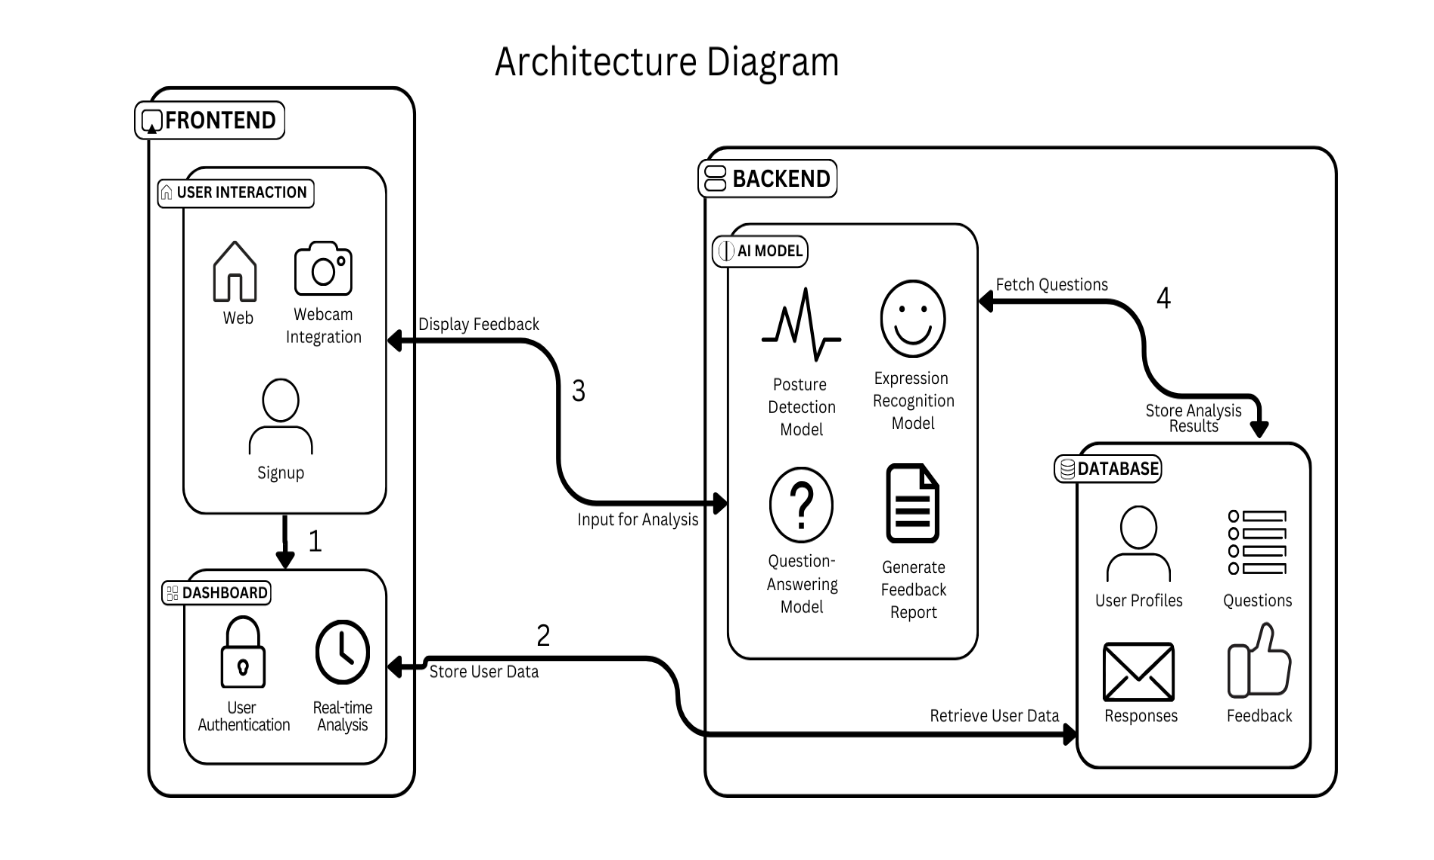
\includegraphics[width=0.8\linewidth]{sections/diagrams/ArchitectureDiagram.png}
\caption{System Architecture Diagram}
\label{fig:architecture}
\end{figure}

\begin{figure}[h]
\centering
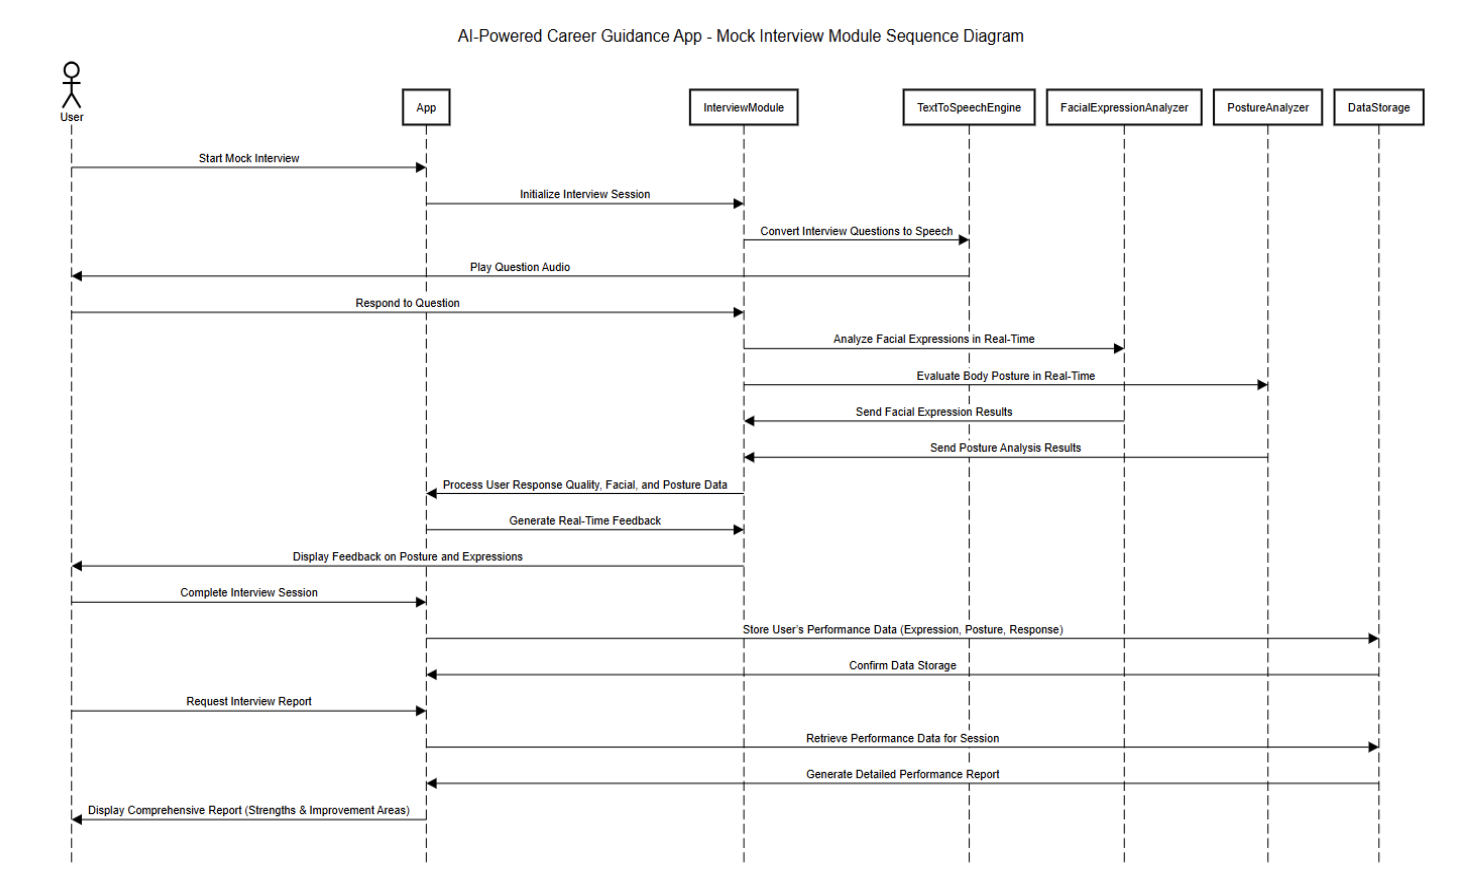
\includegraphics[width=0.8\linewidth]{sections/diagrams/SequentialModel.png}
\caption{Sequential Model Diagram}
\label{fig:sequential}
\end{figure}

\begin{figure}[h]
\centering
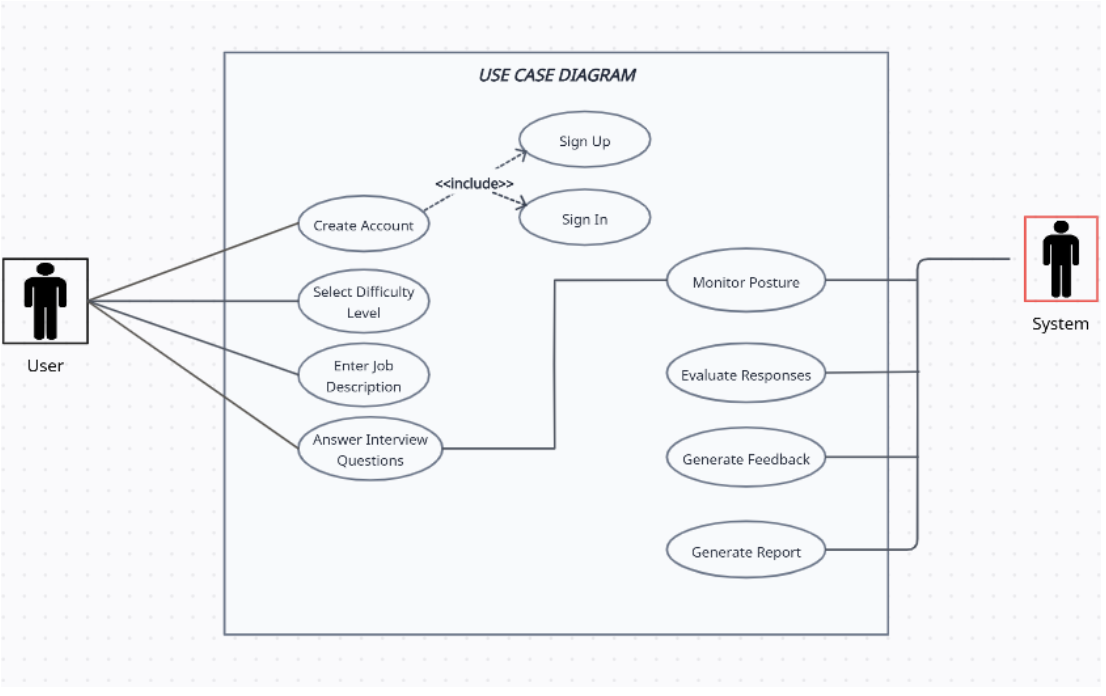
\includegraphics[width=0.8\linewidth]{sections/diagrams/UseCase.png}
\caption{Use Case Diagram}
\label{fig:usecase}
\end{figure}

\begin{figure}[h]
\centering
\begin{tikzpicture}
\begin{umlsystem}[x=4, fill=red!10]{The system}
\umlusecase{Live Interview Analysis}
\umlusecase[y=-2]{Posture Detection}
\umlusecase[y=-4]{Facial Expression Recognition}
\umlusecase[x=4, y=-2, width=1.5cm]{AI Question Generation}
\umlusecase[x=6, fill=green!20]{Interview Scoring}
\umlusecase[x=6, y=-4]{Result Storage}
\end{umlsystem}
\umlactor{User}
\umlactor[y=-3]{Admin}
\umlactor[x=14, y=-1.5]{System}

\umlinherit{Admin}{User}
\umlassoc{User}{usecase-1}
\umlassoc{User}{usecase-2}
\umlassoc{User}{usecase-3}
\umlassoc{System}{usecase-5}
\umlassoc{System}{usecase-6}
\umlinherit{usecase-2}{usecase-1}
\umlVHextend{usecase-5}{usecase-4}
\umlinclude[name=incl]{usecase-3}{usecase-4}
\umlnote[x=7, y=-7]{incl-1}{Real-time AI processing dependency}
\end{tikzpicture}
\caption{Live Interview System Use Case Diagram}
\label{fig:live-interview-usecase}
\end{figure}

---

\chapter{Iteration 2}
\label{ch:iter2}

The second iteration of the HiringGuru project marks a major milestone, targeting the final phase of FYP-1. This chapter presents comprehensive system design artifacts that guide the real-time mock interview application’s architectural, structural, and behavioral layout. The primary focus remains on enhancing the design quality and AI integration while maintaining consistency in the previously defined system requirements.

\section{Domain Model / Class Diagram}
The domain model conceptualizes the fundamental entities and their relationships within the HiringGuru ecosystem. Core entities such as \texttt{User}, \texttt{Interview}, \texttt{Feedback}, and \texttt{AnalysisResult} are defined alongside their properties and associations. The class diagram provides an abstract blueprint of interactions across the Node.js backend and Next.js frontend, forming the structural basis for the platform. The model was collaboratively designed and version-controlled through GitHub at: \textbf{\url{https://github.com/12Samad/FYP-HiringGuru}}.

\section{Component Diagram}
The component diagram breaks down the modular architecture of HiringGuru. It captures the interplay between critical system components including:
\begin{itemize}
    \item Node.js backend and API routing
    \item Next.js frontend styled with TailwindCSS
    \item Posture analysis using MobileNetV2 and MediaPipe
    \item Facial expression detection via Haarcascade
    \item OpenAI GPT integration for dynamic question generation
\end{itemize}
It also illustrates the hybrid posture analysis model leveraging both TensorFlow and MediaPipe for optimized accuracy.

\section{Layer Diagram}
This diagram defines the layered architecture of the system, encompassing:
\begin{itemize}
    \item \textbf{Presentation Layer:} Built with Next.js and TailwindCSS
    \item \textbf{Business Logic Layer:} Implemented in Node.js
    \item \textbf{AI Analysis Layer:} Powered by TensorFlow, OpenCV, Dlib, and MediaPipe
    \item \textbf{Data Access Layer:} Connected via Firebase for real-time data sync
\end{itemize}
This separation ensures maintainability and clarity across the technology stack.

\section{Structure Chart}
The structure chart presents the control flow hierarchy, starting from the user interface, down to the analysis modules such as posture, facial expression, and eye contact detection. It reflects how responsibilities are distributed across frontend, backend, and AI services. The Python-based Text-to-Speech (TTS) engine is also integrated at this layer.

\textbf{Behavioral Design}

\section{Flow Diagram}
The system flow diagram visualizes the end-to-end journey from user login to interview execution and final feedback generation. It highlights the real-time interaction pipeline involving:
\begin{itemize}
    \item Question generation via OpenAI
    \item Posture detection (MobileNetV2 + MediaPipe)
    \item Facial and eye analysis (Haarcascade, Dlib)
    \item Feedback persistence in Firebase
\end{itemize}

\section{Data Flow Diagram (DFD)}
The DFD maps data sources, processes, and destinations in HiringGuru. Key elements include:
\begin{itemize}
    \item Inputs: Webcam stream, user data
    \item Processing: Posture/facial/eye tracking using AI models
    \item Outputs: Feedback reports stored in Firebase
\end{itemize}

\section{Data Dictionary}
The data dictionary documents all entities, attributes, and relationships within the application. Important structures include:
\begin{itemize}
    \item \texttt{User}: ID, name, email
    \item \texttt{Interview}: Timestamp, question set
    \item \texttt{AnalysisResult}: Posture metrics, facial scores, eye contact duration
    \item \texttt{Feedback}: Comments, suggestions, ratings
\end{itemize}

\section{Activity Diagram}
This diagram captures the lifecycle of a mock interview session, beginning from user authentication and culminating in feedback delivery. It also emphasizes image processing steps like grayscale transformation via OpenCV before AI inference.

\section{State Machine Diagram}
The state diagram models behavioral transitions such as:
\begin{itemize}
    \item Waiting for User
    \item Posture Analysis in Progress
    \item Facial Recognition Active
    \item Question Generation via OpenAI
    \item Feedback Summary Display
\end{itemize}

\section{Sequence Diagram}
The sequence diagram outlines the message flow across system components:
\begin{itemize}
    \item Request-response cycles between Next.js UI and Node.js server
    \item Real-time analysis using TensorFlow and OpenCV
    \item Integration with Firebase for data storage
    \item Dynamic questions fetched from OpenAI API
\end{itemize}

\section{Interaction Overview Diagram}
This diagram merges sequence and activity views, detailing AI model interactions (MobileNetV2, Haarcascade, Dlib) and their orchestration through the central backend with Firebase and frontend interfaces.

\section{Entity-Relationship (ER) Diagram}
The ER diagram reflects the Firebase database schema, mapping entities like \texttt{Users}, \texttt{Interviews}, and \texttt{AnalysisResults}. This design facilitates efficient data access and storage of AI-generated insights.

\section{Data Structure Design}
Data structures were carefully selected to support real-time processing. Key choices include:
\begin{itemize}
    \item JSON-based data exchange
    \item Array structures for time-series posture metrics
    \item Object models for feedback and facial metrics
\end{itemize}

\section{Algorithm Design}
The algorithmic core of HiringGuru includes:
\begin{itemize}
    \item \textbf{Posture Analysis:} MobileNetV2 achieving 90\% accuracy
    \item \textbf{Facial Detection:} Haarcascade frontal face model
    \item \textbf{Eye Contact Tracking:} Dlib’s frontal face detector
    \item \textbf{Question Generation:} OpenAI GPT model with prompt tuning
\end{itemize}
The hybrid model using MediaPipe boosts reliability in varied lighting and camera angles.

\section{Development Phase}
The development phase strictly follows clean code principles with:
\begin{itemize}
    \item Modular folder structure
    \item Clear variable and function naming conventions
    \item Integrated ESLint and Prettier for static code analysis
\end{itemize}
All code is versioned and maintained on GitHub: \textbf{\url{https://github.com/12Samad/FYP-HiringGuru}}.

\subsection{Unit Tests}
Unit testing ensures the reliability of each module independently:
\begin{itemize}
    \item MobileNetV2 posture model
    \item Haarcascade facial analysis
    \item Dlib-based eye tracking
    \item OpenAI question generation API
\end{itemize}

\subsection{Test Suites and Test Cases}
Test cases are defined to cover all edge scenarios, especially in the AI feedback loop. These validate model performance, frontend input handling, and backend API response integrity.

\subsubsection{Authentication Test Cases}
\begin{table}[!htbp]
    \centering
    \begin{tabular}{|c|p{6cm}|c|c|}
        \hline
        \textbf{Test Case ID} & \textbf{Description} & \textbf{Expected Output} & \textbf{Iteration} \\
        \hline
        TC-A1 & Login with valid email and password & User is logged in & 1 \\
        \hline
        TC-A2 & Login with invalid password & Error message is shown & 1 \\
        \hline
        TC-A3 & Attempt login with unregistered email & Account not found message & 1 \\
        \hline
        TC-A4 & Password encryption test & Password is securely hashed & 1 \\
        \hline
    \end{tabular}
    \caption{Authentication Test Cases}
    \label{tab:auth-test-cases}
\end{table}


\subsubsection{Posture Detection Test Cases}
\begin{table}[!htbp]
    \centering
    \begin{tabular}{|c|p{6cm}|c|c|}
        \hline
        \textbf{Test Case ID} & \textbf{Description} & \textbf{Expected Output} & \textbf{Iteration} \\
        \hline
        TC-P1 & Detect good posture in real-time & System identifies correct posture & 2 \\
        \hline
        TC-P2 & Detect slouching posture & System alerts user of bad posture & 2 \\
        \hline
        TC-P3 & Switch between postures rapidly & System adapts to changes smoothly & 2 \\
        \hline
        TC-P4 & No user in front of camera & System disables detection & 2 \\
        \hline
    \end{tabular}
    \caption{Posture Detection Test Cases}
    \label{tab:posture-test-cases}
\end{table}


\subsubsection{System Behavior and Performance Test Cases}
\begin{table}[!htbp]
    \centering
    \begin{tabular}{|c|p{6cm}|c|c|}
        \hline
        \textbf{Test Case ID} & \textbf{Description} & \textbf{Expected Output} & \textbf{Iteration} \\
        \hline
        TC-S1 & System start-up time & App loads within 5 seconds & 3 \\
        \hline
        TC-S2 & CPU usage under load & CPU usage remains below 60\% & 3 \\
        \hline
        TC-S3 & Real-time alerts responsiveness & Alerts are shown within 1 second & 3 \\
        \hline
        TC-S4 & Application memory usage & Memory footprint under 200MB & 3 \\
        \hline
    \end{tabular}
    \caption{System Behavior and Performance Test Cases}
    \label{tab:system-performance-test-cases}
\end{table}


\section{Maintainable Phase}

\subsection{CI/CD}
A GitHub Actions pipeline is used for automated testing and deployment. CI ensures clean integration across contributors while CD streamlines model and feature rollout.

\subsection{Deployment Diagram}
This diagram illustrates cloud and local infrastructure for Hosting (Vercel), AI model servers (local/Python environment), Firebase (Realtime Database), and Node.js services running Express.js.

\subsection{System-Level Test Suites}
System-level testing is conducted to ensure complete functional integration:
\begin{itemize}
    \item Cross-layer interactions (Frontend ↔ Backend ↔ Firebase)
    \item Real-time analysis data streaming
    \item Consistent UI behavior under AI feedback changes
\end{itemize}

\subsection{Version Control (GitHub)}
HiringGuru uses GitHub for collaboration and revision control. Repository: \textbf{\url{https://github.com/12Samad/FYP-HiringGuru}}.

\subsection{Configuration / Tool Setup Manual}
Environment setup involves:
\begin{itemize}
    \item Node.js and Next.js installation
    \item TailwindCSS configuration
    \item TensorFlow, MediaPipe, and OpenCV setup
    \item Firebase SDK initialization
    \item OpenAI API key integration
\end{itemize}
The full setup instructions are available in the GitHub repository’s \texttt{README.md} file.

\section{Relevant Diagrams}
\begin{figure}[h]
\centering
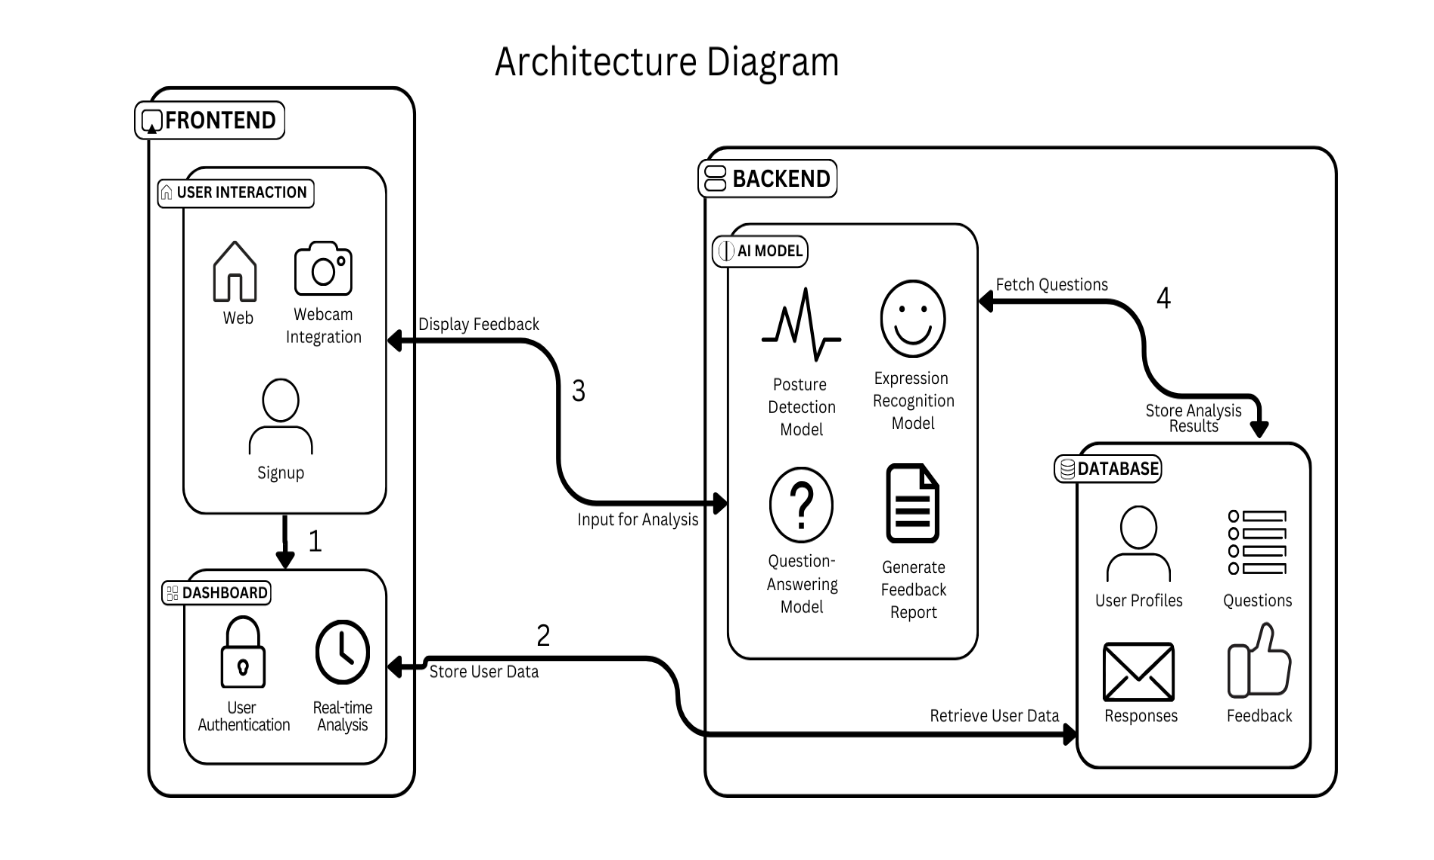
\includegraphics[width=0.8\linewidth]{sections/diagrams/ArchitectureDiagram.png}
\caption{System Architecture Diagram}
\label{fig:architecture}
\end{figure}

\begin{figure}[h]
\centering
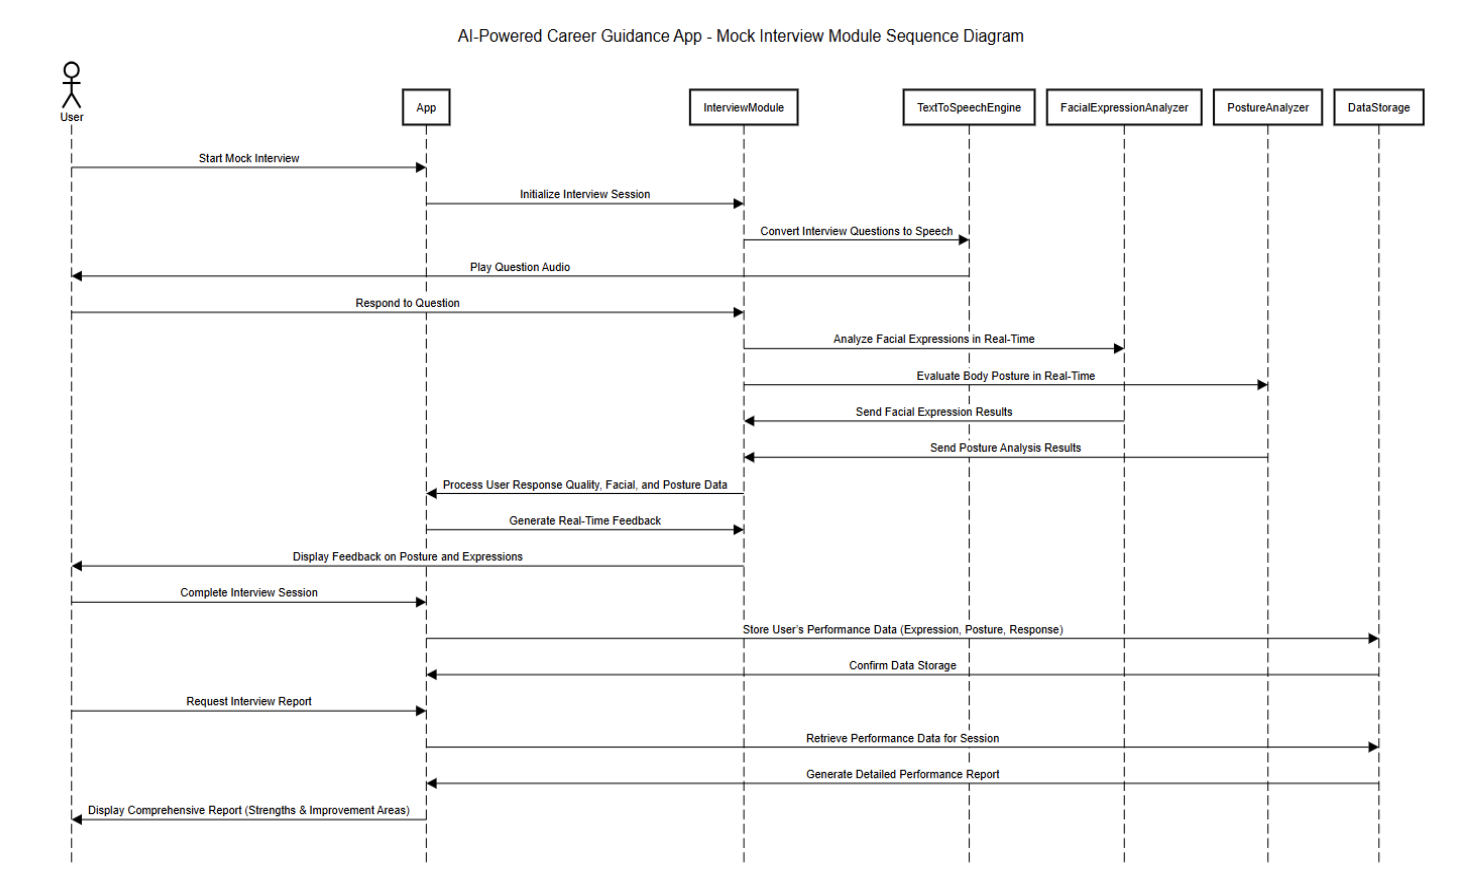
\includegraphics[width=0.8\linewidth]{sections/diagrams/SequentialModel.png}
\caption{Sequential Model Diagram}
\label{fig:sequential}
\end{figure}

\begin{figure}[h]
\centering
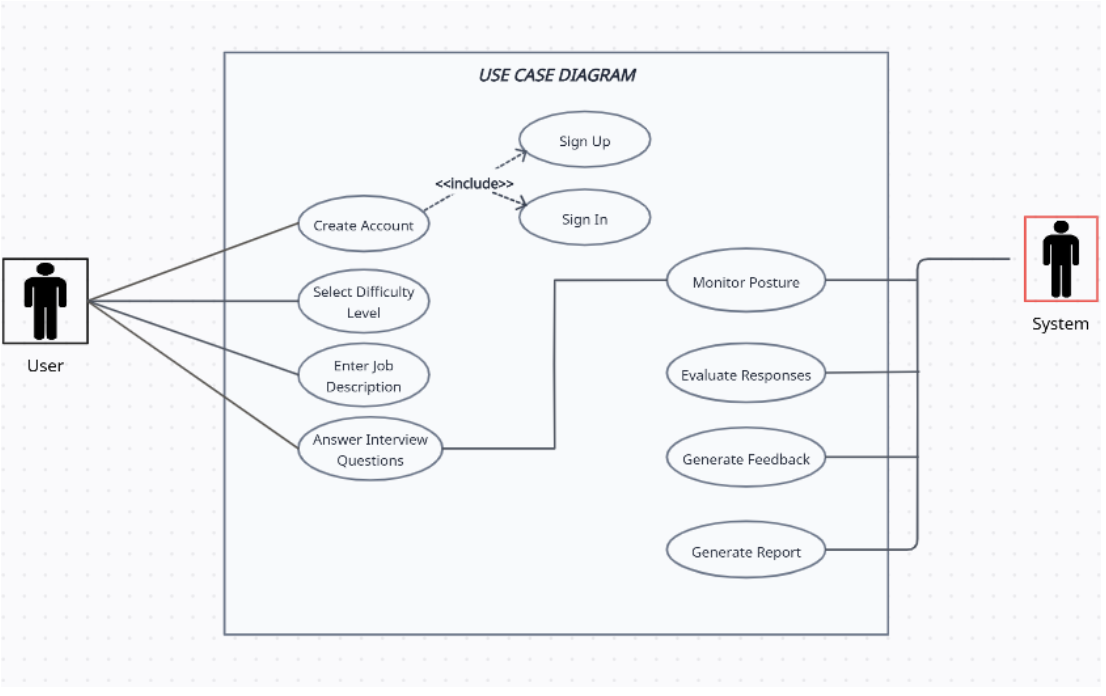
\includegraphics[width=0.8\linewidth]{sections/diagrams/UseCase.png}
\caption{Use Case Diagram}
\label{fig:usecase}
\end{figure}

\chapter{Iteration 3}
\label{ch:iter3}

The third iteration of \textbf{HiringGuru} was planned for completion around the midterm of FYP-2. This chapter outlines the core design and testing activities conducted during this phase, focusing on the structural and behavioral aspects of the system. While the functional requirements remained consistent, the system architecture evolved to support a robust, scalable, and maintainable real-time mock interview platform with integrated AI-based analysis.

\section{Structural Design}

\subsection{Domain Model/Class Diagram}
The domain model defines key entities in the HiringGuru ecosystem, including \texttt{User}, \texttt{Interview}, \texttt{AnalysisResults}, and \texttt{Feedback}. The class diagram illustrates the interaction among components of the Node.js backend, Next.js frontend, and AI modules, showcasing the object-oriented structure of the application.

\subsection{Component Diagram}
The component diagram presents a modular breakdown of HiringGuru’s architecture. It includes:
\begin{itemize}
  \item Backend (Node.js + Express)
  \item Frontend (Next.js + TailwindCSS)
  \item AI Modules: MobileNetV2 (posture detection), MediaPipe (landmark analysis), Haarcascade (facial expression), Dlib (eye tracking)
  \item External APIs: OpenAI for question generation
  \item Database: Firebase Realtime Database
\end{itemize}
These components are designed to work asynchronously and in real-time to ensure a smooth user experience.

\subsection{Layer Diagram}
HiringGuru is structured in a layered architecture:
\begin{itemize}
  \item \textbf{Presentation Layer:} Next.js with TailwindCSS
  \item \textbf{Business Logic Layer:} Node.js backend handling APIs and middleware
  \item \textbf{AI Analysis Layer:} TensorFlow, OpenCV (CV2), MediaPipe, Dlib
  \item \textbf{Data Access Layer:} Firebase Realtime Database
\end{itemize}

\subsection{Structure Chart}
The structure chart showcases the hierarchical module organization: from the core interview engine and voice synthesis module (Python TTS) to AI-based analytics modules, including posture and facial tracking subsystems. The AI modules achieve over 90\% accuracy in posture analysis.

\section{Behavior Design}

\subsection{Flow Diagram}
The flow diagram depicts the end-to-end user journey, beginning with Firebase-based authentication, progressing through the interview session, AI-powered analysis, and real-time feedback presentation.

\subsection{Data Flow Diagram (DFD)}
The DFD visualizes how webcam input is processed:
\begin{itemize}
  \item Captured via browser
  \item Converted to grayscale using CV2
  \item Fed into trained AI models (e.g., MobileNetV2, MediaPipe)
  \item Results are stored in Firebase and displayed via the frontend
\end{itemize}

\subsection{Data Dictionary}
The data dictionary defines elements such as:
\begin{itemize}
  \item \texttt{User}: \texttt{name}, \texttt{email}, \texttt{role}
  \item \texttt{Interview}: \texttt{sessionId}, \texttt{timestamp}, \texttt{questions}
  \item \texttt{AnalysisResults}: posture accuracy, facial expression score, eye tracking metrics
  \item \texttt{Feedback}: timestamp, suggestions, scores
\end{itemize}

\subsection{Activity Diagram}
The activity diagram demonstrates the interview process lifecycle:
\begin{enumerate}
  \item Session initialization
  \item Dynamic question generation via OpenAI API
  \item Real-time AI analysis and user monitoring
  \item Feedback generation and session summary
\end{enumerate}

\subsection{State Machine Diagram}
The state machine tracks session transitions, such as:
\begin{itemize}
  \item \texttt{Idle} → \texttt{Recording} (user starts interview)
  \item \texttt{Recording} → \texttt{Analyzing} (frame-by-frame AI analysis)
  \item \texttt{Analyzing} → \texttt{Feedback} (session ends, data summarized)
\end{itemize}

\subsection{Sequence Diagram}
The sequence diagram details interactions between:
\begin{itemize}
  \item Next.js frontend
  \item Node.js backend API
  \item Firebase Database
  \item TensorFlow and Python-based AI scripts
\end{itemize}
This flow ensures minimal latency during real-time analysis.

\subsection{Interaction Overview Diagram}
A high-level integration of activity and sequence diagrams, showing how frontend UI triggers backend processes, feeds into AI models, and synchronizes data with Firebase for feedback display.

\section{Schema Design / ER Diagram}
The ER diagram maps Firebase collections and their attributes, including:
\begin{itemize}
  \item \texttt{Users}: UID, Email, Role
  \item \texttt{Interviews}: InterviewID, Timestamp, UserID
  \item \texttt{AnalysisResults}: InterviewID, FrameMetrics, TimeLogs
  \item \texttt{Feedback}: InterviewID, Suggestions, Final Scores
\end{itemize}

\section{Data Structure Design}
Key data structures include:
\begin{itemize}
  \item \textbf{Arrays:} Frame-wise AI results
  \item \textbf{Objects:} User sessions, interview metadata
  \item \textbf{Dictionaries/Maps:} Real-time feedback and error handling
\end{itemize}

\section{Algorithm Design}
HiringGuru incorporates multiple AI algorithms:
\begin{itemize}
  \item \textbf{Posture Analysis:} MobileNetV2 achieving ~90\% accuracy
  \item \textbf{Face Tracking:} Haarcascade classifiers
  \item \textbf{Eye Movement:} Dlib-based shape prediction
  \item \textbf{Question Generation:} OpenAI GPT-based prompts
\end{itemize}

\section{Development Phase}
\begin{itemize}
  \item \textbf{Coding Standards:} ESLint and Prettier for Node.js/Next.js
  \item \textbf{Styling:} TailwindCSS for consistency and responsiveness
  \item \textbf{Static Analysis:} Integration of linters and testing tools
\end{itemize}

\subsection{Unit Tests}
\begin{table}[!htbp]
\centering
\begin{tabular}{|c|p{8cm}|c|}
\hline
\textbf{Test Case ID} & \textbf{Description} & \textbf{Expected Output} \\
\hline
UT-01 & Validate OpenAI API returns relevant question set & Accurate questions displayed \\
\hline
UT-02 & Ensure AI posture analysis handles bad frames & Graceful fallback, no crash \\
\hline
\end{tabular}
\caption{Sample Unit Test Cases}
\label{tab:unit-test-cases}
\end{table}

\subsection{Test Suites}
Test suites include:
\begin{itemize}
  \item Functional Testing: Core interview features
  \item Integration Testing: Backend-AI-Firebase communication
  \item Regression Testing: Post feature addition
\end{itemize}

\section{Maintainable Phase}

\subsection{CI/CD}
CI/CD pipeline is integrated with GitHub Actions:
\begin{itemize}
  \item Automated builds and test execution
  \item Deployment to Vercel (frontend) and Firebase (backend + DB)
\end{itemize}

\subsection{Deployment Diagram}
The deployment diagram shows:
\begin{itemize}
  \item Next.js frontend hosted on Vercel
  \item Node.js backend deployed via Firebase Functions
  \item Firebase Realtime Database for persistent storage
  \item External AI scripts running on local Python services
\end{itemize}

\subsection{System-Level Tests}
\begin{table}[!htbp]
\centering
\begin{tabular}{|c|p{8cm}|c|}
\hline
\textbf{Test Case ID} & \textbf{Description} & \textbf{Expected Output} \\
\hline
ST-01 & End-to-end login and session initiation & Successful login and interview load \\
\hline
ST-02 & Data storage for every second/frame & Data logged and stored in Firebase \\
\hline
\end{tabular}
\caption{System-Level Test Cases}
\label{tab:system-test-cases}
\end{table}

\subsection{GitHub Repository}
All source code and documentation are maintained in the following GitHub repository:  
\textbf{\url{https://github.com/12Samad/FYP-HiringGuru}}

\subsection{Setup and Tool Manual}
HiringGuru setup requires:
\begin{itemize}
  \item Node.js, Next.js, and TailwindCSS
  \item Python 3.x with TensorFlow, OpenCV, MediaPipe, Dlib
  \item Firebase project setup and environment configuration
  \item OpenAI API key for dynamic question generation
\end{itemize}

\section{UML Use Case Diagram}
\begin{figure}[h]
  \centering
  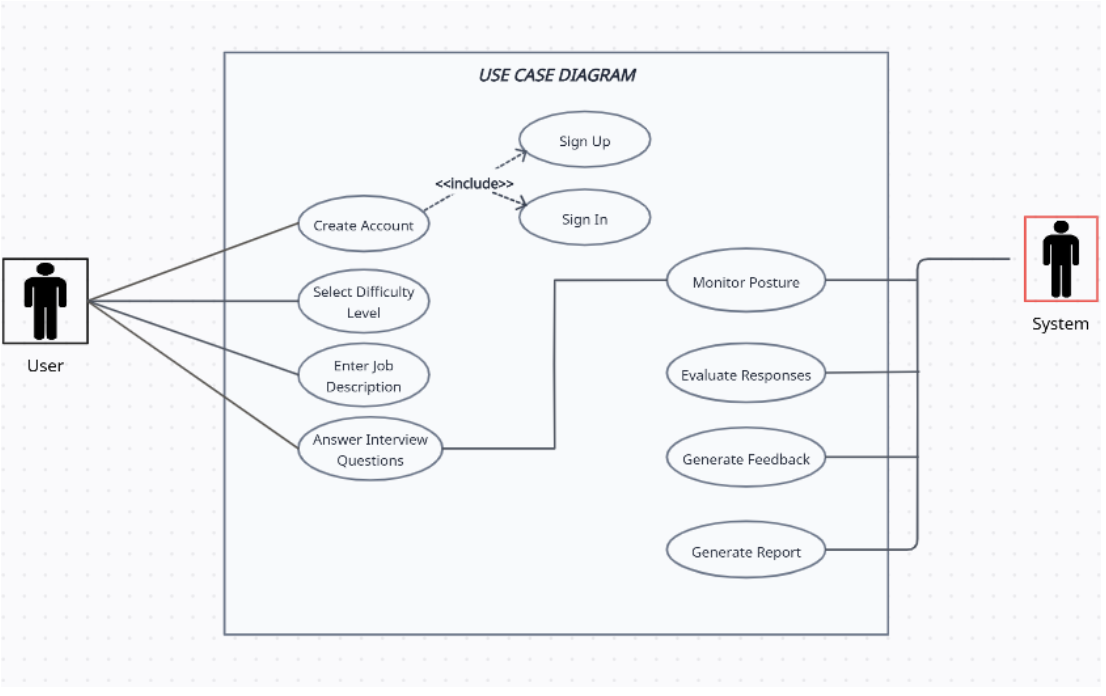
\includegraphics[width=0.8\textwidth]{sections/diagrams/UseCase.png}
  \caption{UML Use Case Diagram for HiringGuru}
  \label{fig:use-case}
\end{figure}

This chapter documents the design, implementation, and testing strategies that contributed to a functional and scalable version of HiringGuru by Iteration 3. The combination of web technologies and AI modules has laid a solid foundation for continued development and refinement of the real-time mock interview platform.


\chapter{Iteration 4}
\label{ch:iter4}

This chapter documents the fourth iteration of HiringGuru, completed during the final phase of FYP-2. It focuses on the system design artifacts, detailing structural and behavioral aspects of the real-time mock interview platform. While the requirements analysis remains consistent across iterations, this phase emphasizes the design, development, and testing of HiringGuru’s architecture and components.

\section{Structural Design}

\subsection{Domain Model and Class Diagram}
The \textbf{Domain Model} outlines the conceptual structure of HiringGuru, defining core entities such as \texttt{User}, \texttt{Interview}, \texttt{AnalysisResults}, and \texttt{Feedback}, along with their relationships. For example, a \texttt{User} can participate in multiple \texttt{Interview} sessions, each generating \texttt{AnalysisResults} and \texttt{Feedback}. The \textbf{Class Diagram} provides a static view of the system, detailing classes like \texttt{UserProfile} (attributes: userID, email, name), \texttt{InterviewSession} (attributes: sessionID, timestamp, duration), and \texttt{AIAnalysis} (methods: analyzePosture(), detectExpression()). It illustrates associations between the Next.js frontend, Node.js backend, and AI analysis modules, ensuring a cohesive design.

\subsection{Component Diagram}
The \textbf{Component Diagram} depicts HiringGuru’s modular components: the Next.js frontend styled with TailwindCSS, the Node.js backend for business logic, AI analysis modules (MobileNetV2 for posture detection \cite{howard2018mobilenetv2}, MediaPipe for landmark tracking \cite{lugaresi2019mediapipe}, Haarcascade for facial expressions \cite{viola2001haar}, Dlib for eye tracking \cite{king2009dlib}), Python TTS for voice conversion, and Firebase for real-time data storage \cite{firebase2023docs}. It highlights interfaces and dependencies, such as the backend’s reliance on Firebase for user authentication and session data.

\subsection{Layer Diagram}
The \textbf{Layer Diagram} organizes HiringGuru into four distinct layers:
\begin{itemize}
    \item \textbf{Presentation Layer}: Next.js with TailwindCSS delivers a responsive user interface \cite{vercel2023nextjs}.
    \item \textbf{Business Logic Layer}: Node.js handles interview session management and API coordination.
    \item \textbf{AI Analysis Layer}: TensorFlow, MediaPipe, and OpenCV (CV2) process webcam input for real-time feedback.
    \item \textbf{Data Access Layer}: Firebase manages user data, session logs, and analysis results.
\end{itemize}
This layered architecture ensures scalability and maintainability by isolating responsibilities.

\subsection{Structure Chart}
The \textbf{Structure Chart} illustrates the hierarchical organization of HiringGuru’s modules, including the core interview system, OpenAI API for question generation \cite{openai2023api}, Python TTS for voice output, and AI analysis components (posture detection with 90\% accuracy, facial expression analysis, eye tracking). It maps the flow of control, showing function calls between modules, such as the backend invoking AI analysis during an interview session.

\section{Behavioral Design}

\subsection{Flow Diagram}
The \textbf{Flow Diagram} outlines the operational sequence of HiringGuru: user authentication via Firebase, interview setup, real-time AI analysis (posture, facial expressions, eye tracking), question generation using the OpenAI API, and feedback delivery. It emphasizes the seamless integration of AI modules to provide immediate, actionable insights during mock interviews.

\subsection{Data Flow Diagram (DFD)}
The \textbf{Data Flow Diagram (DFD)} models the flow of data within HiringGuru. Key processes include webcam input preprocessing (using CV2 for grayscaling), AI analysis (MobileNetV2 for posture, Haarcascade for facial expressions, Dlib for eye tracking), and storage in Firebase. External entities like users interact with the system, while data stores (Firebase database) manage session logs and analysis results.

\subsection{Data Dictionary}
The \textbf{Data Dictionary} defines HiringGuru’s data elements:
\begin{itemize}
    \item \texttt{User}: Attributes (userID: string, email: string, name: string).
    \item \texttt{Interview}: Attributes (sessionID: string, timestamp: datetime, duration: integer).
    \item \texttt{AnalysisResults}: Attributes (sessionID: string, postureScore: float, expressionData: string, eyeContactStats: float).
    \item \texttt{Feedback}: Attributes (feedbackID: string, sessionID: string, suggestions: string).
\end{itemize}
Each entry specifies data types, constraints, and relationships, ensuring clarity in data management.

\subsection{Activity Diagram}
The \textbf{Activity Diagram} models the workflow of a mock interview session, including user authentication, interview initialization, real-time analysis (posture, facial expressions, eye tracking), question delivery, and feedback generation. Decision nodes handle scenarios like posture correction prompts if MobileNetV2 detects improper alignment.

\subsection{State Machine Diagram}
The \textbf{State Machine Diagram} defines the states of an interview session: ``Idle'', ``Authenticating'', ``Analyzing Posture'', ``Detecting Facial Expressions'', ``Tracking Eye Contact'', ``Generating Questions'', and ``Providing Feedback''. Transitions occur based on events such as posture changes (detected by MobileNetV2 \cite{howard2018mobilenetv2}) or question delivery (via OpenAI API \cite{openai2023api}).

\subsection{Sequence Diagram}
The \textbf{Sequence Diagram} illustrates interactions during an interview session, showing message exchanges between the Next.js frontend, Node.js backend, AI analysis modules (TensorFlow, MediaPipe, CV2, Dlib), OpenAI API, and Firebase database. It details the sequence of operations, such as initiating an interview, processing webcam input, and storing results.

\subsection{Interaction Overview Diagram}
The \textbf{Interaction Overview Diagram} provides a high-level view of HiringGuru’s interactions, combining elements of sequence and activity diagrams. It focuses on coordination between AI analysis modules and core components, ensuring efficient data flow and feedback delivery.

\section{Schema Design: ER Diagram}
The \textbf{Entity-Relationship (ER) Diagram} models HiringGuru’s Firebase database structure, defining entities like \texttt{Users} (attributes: userID, email, name), \texttt{Interviews} (attributes: sessionID, userID, timestamp), \texttt{AnalysisResults} (attributes: sessionID, postureScore, expressionData, eyeContactStats), and \texttt{Feedback} (attributes: feedbackID, sessionID, suggestions). Relationships include a one-to-many mapping between \texttt{Users} and \texttt{Interviews}, ensuring efficient data retrieval.

\section{Data Structure Design}
The \textbf{Data Structure Design} outlines data organization in HiringGuru: arrays store real-time posture and expression analysis results, JSON objects manage user profiles and interview sessions, and Firebase-optimized structures enable fast queries for session logs and feedback. This design ensures efficient storage and retrieval of AI-generated data.

\section{Algorithm Design}
This section details the key algorithms in HiringGuru:
\begin{itemize}
    \item \textbf{MobileNetV2}: Performs real-time posture detection with 90\% accuracy \cite{howard2018mobilenetv2}.
    \item \textbf{MediaPipe}: Provides lightweight, high-precision landmark tracking for enhanced posture detection \cite{lugaresi2019mediapipe}.
    \item \textbf{Haarcascade}: Detects facial expressions using pre-trained cascades \cite{viola2001haar}.
    \item \textbf{Dlib}: Tracks eye contact via facial landmark detection \cite{king2009dlib}.
    \item \textbf{OpenAI API}: Generates contextually relevant interview questions based on user profiles \cite{openai2023api}.
\end{itemize}
These algorithms are optimized for low-latency performance and integrated into HiringGuru’s AI analysis pipeline.

\section{Development Phase}
This phase enforces coding standards across HiringGuru’s components, including camelCase for variables (e.g., \texttt{userProfile}), PascalCase for classes (e.g., \texttt{AIAnalysis}), and inline comments for clarity. Static analysis tools like ESLint (for JavaScript) and Pylint (for Python) ensure code quality in the Next.js frontend, Node.js backend, and AI modules.

\subsection{Unit Testing}
Unit tests validate individual components of HiringGuru, ensuring reliability:

\begin{table}[!htbp]
\centering
\begin{tabular}{|c|p{6cm}|c|}
\hline
\textbf{Test Case ID} & \textbf{Description} & \textbf{Expected Output} \\
\hline
UT-01 & Verify posture detection with MobileNetV2 & Correct posture score returned \\
\hline
UT-02 & Test facial expression detection with Haarcascade & Accurate expression classification \\
\hline
UT-03 & Validate eye tracking with Dlib & Correct eye contact statistics \\
\hline
UT-04 & Ensure OpenAI API generates relevant questions & Contextually appropriate questions returned \\
\hline
\end{tabular}
\caption{Unit Test Cases for Iteration 4}
\label{tab:unit-test-cases}
\end{table}

\subsection{Test Suites}
Test suites encompass functional testing (e.g., interview workflow), integration testing (e.g., coordination between AI modules and backend), and regression testing after updates. Test cases address edge scenarios, such as low-light conditions affecting webcam input or errors in question generation.

\section{Maintainable Phase}

\subsection{CI/CD Pipeline}
\textbf{Continuous Integration and Continuous Deployment (CI/CD)} is implemented using GitHub Actions, automating unit and integration tests on code commits and deploying updates to the production environment. This ensures rapid iteration and high code quality throughout development.

\subsection{Deployment Diagram}
The \textbf{Deployment Diagram} illustrates HiringGuru’s infrastructure: Node.js servers are hosted on a cloud platform, Firebase provides real-time database and authentication services \cite{firebase2023docs}, TensorFlow models are deployed on edge devices for efficient AI analysis, and the Next.js frontend is served via a CDN for low-latency access.

\subsection{System-Level Testing}
System-level tests validate HiringGuru’s end-to-end functionality:

\begin{table}[!htbp]
\centering
\begin{tabular}{|c|p{6cm}|c|}
\hline
\textbf{Test Case ID} & \textbf{Description} & \textbf{Expected Output} \\
\hline
ST-01 & Verify end-to-end interview session workflow & User completes session with feedback \\
\hline
ST-02 & Ensure real-time analysis under varying network conditions & Analysis results remain accurate \\
\hline
ST-03 & Validate Firebase data consistency after session & All session data stored correctly \\
\hline
ST-04 & Test system scalability with 100 concurrent users & System handles load without crashes \\
\hline
\end{tabular}
\caption{System-Level Test Cases for Iteration 4}
\label{tab:system-test-cases}
\end{table}

\subsection{Version Control }
Version control is managed via \textbf{GitHub}, facilitating collaboration and change tracking across HiringGuru’s components. Access at: \url{https://github.com/12Samad/FYP-HiringGuru}.

\subsection{Configuration and Setup Manual (Optional)}
This section outlines setup instructions for HiringGuru:
\begin{itemize}
    \item \textbf{Dependencies}: Install Node.js, Next.js, TensorFlow, MediaPipe, OpenCV, and Dlib.
    \item \textbf{API Configuration}: Set up OpenAI API keys for question generation \cite{openai2023api}.
    \item \textbf{Database}: Configure Firebase for authentication and real-time database \cite{firebase2023docs}.
    \item \textbf{Deployment}: Deploy the Next.js frontend via a CDN and Node.js backend on a cloud platform.
\end{itemize}
A tool manual covers usage of development tools like VS Code, ESLint, and GitHub Actions.

\section{UML Use Case Diagram}
\begin{figure}[h]
  \centering
  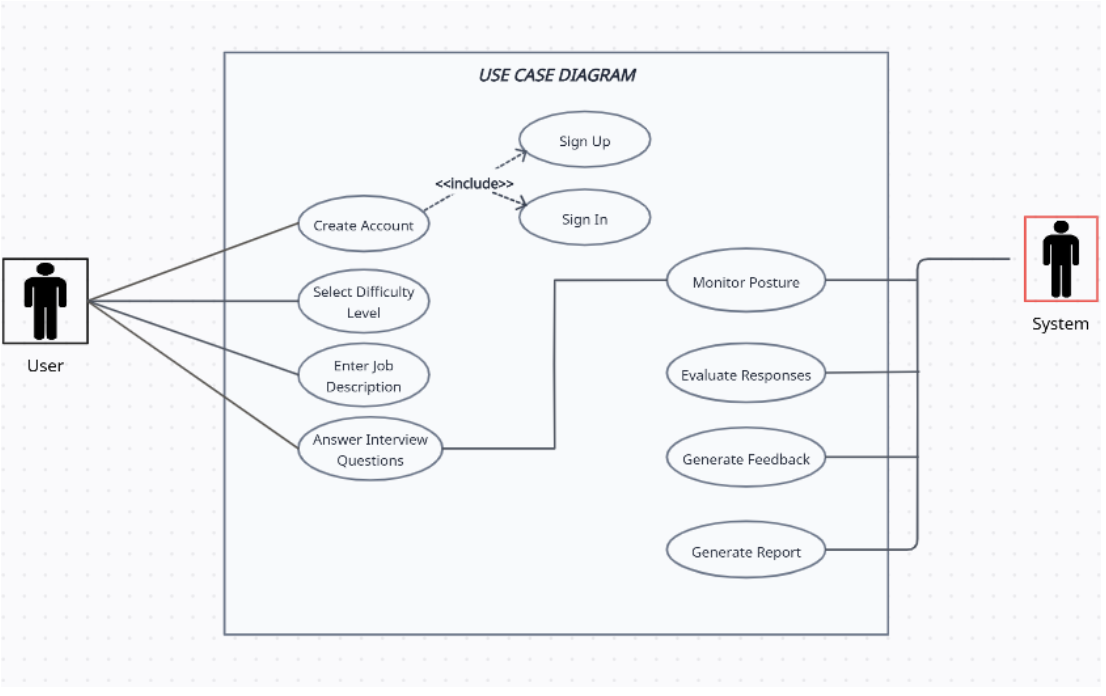
\includegraphics[width=0.8\textwidth]{sections/diagrams/UseCase.png}
  \caption{UML Use Case Diagram for HiringGuru}
  \label{fig:use-case}
\end{figure}

This chapter provides a comprehensive overview of Iteration 4, detailing the design, development, and testing of HiringGuru. The artifacts ensure a robust, maintainable platform with advanced AI-driven feedback capabilities for real-time mock interviews.
\chapter{Implementation Details}
\label{ch:implementation}

This chapter elaborates on the algorithmic and procedural backbone of HiringGuru, focusing on backend processes and integration strategies that ensure operational integrity. Key workflows, system interactions, and validation mechanisms are discussed to demonstrate the robustness of the real-time mock interview platform.

%---------------------------------------------------------------------
\section{Core Algorithmic Workflows}
HiringGuru relies on several critical algorithms and processes to deliver AI-driven interview feedback:

\subsection{Authentication Protocol}
The authentication mechanism uses Firebase Authentication, leveraging secure token-based access with JSON Web Tokens (JWT) for session management (Figure~\ref{fig:architecture}). User credentials are hashed using bcrypt, ensuring no plaintext storage. The workflow verifies user identity and authorizes access to interview sessions.

\subsection{Real-Time Analysis Pipeline}
The pipeline processes webcam input for posture, facial expression, and eye contact analysis:
\begin{itemize}
    \item \textbf{Step 1}: Webcam frames are preprocessed using OpenCV (CV2) for grayscaling and noise reduction.
    \item \textbf{Step 2}: MobileNetV2 and MediaPipe analyze posture, achieving 90\% accuracy, while Haarcascade and Dlib handle facial expression and eye contact detection, respectively.
    \item \textbf{Step 3}: Analysis results are aggregated and stored in Firebase for real-time feedback generation.
\end{itemize}

\subsection{Question Generation Workflow}
The OpenAI API generates contextually relevant interview questions based on user profiles and job roles. Questions are cached in memory to minimize API calls, ensuring low-latency delivery during interview sessions.

%---------------------------------------------------------------------
\section{System Interaction Model}
Figure~\ref{fig:sequential-model} illustrates the sequential processing of user interactions, from authentication to feedback delivery. The UML Use Case Diagram below details actor-use case relationships, highlighting the interactions between users and the system.

\begin{figure}[h]
  \centering
  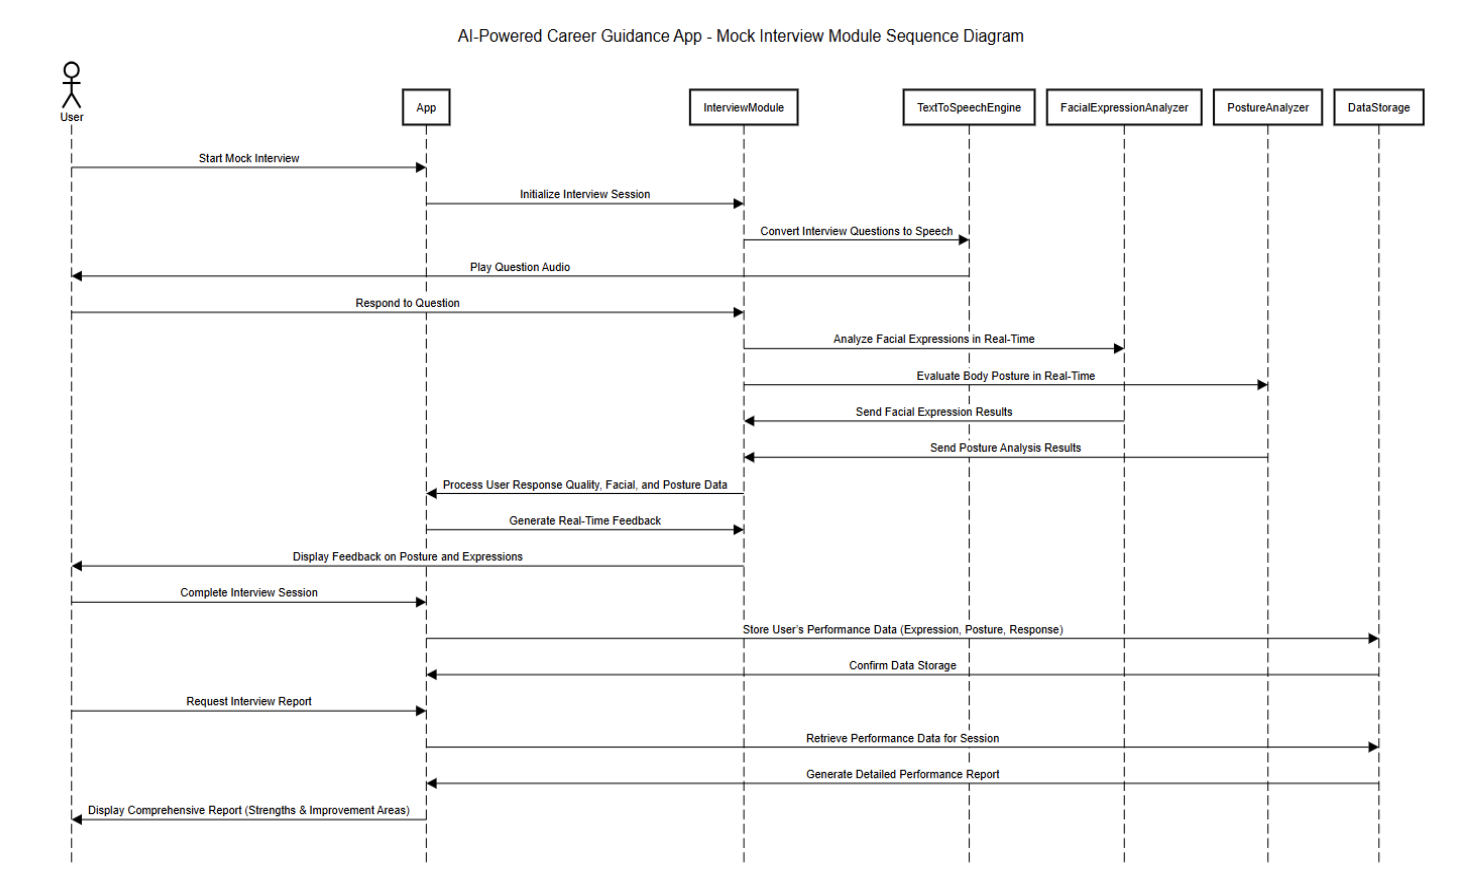
\includegraphics[width=0.9\textwidth]{sections/diagrams/SequentialModel.png}
  \caption{Sequential processing model for user requests}
  \label{fig:sequential-model}
\end{figure}

% UML Use Case Diagram for HiringGuru
\begin{figure}[h]
\centering
\begin{tikzpicture}
% System Boundary
\begin{umlsystem}[x=4, fill=blue!5]{HiringGuru}
  \umlusecase[name=startInterview, x=2, y=0]{Start Interview}
  \umlusecase[name=analyzePosture, x=2, y=-2]{Analyze Posture}
  \umlusecase[name=generateFeedback, x=2, y=-4]{Generate Feedback}
  \umlusecase[name=manageQuestions, x=6, y=-2]{Manage Questions}
\end{umlsystem}

% Actors
\umlactor[x=-2, y=0]{User}
\umlactor[x=12, y=-2]{Admin}

% Relationships
\umlassoc{User}{startInterview}
\umlassoc{Admin}{manageQuestions}
\umlinclude{startInterview}{analyzePosture}
\umlVHextend{generateFeedback}{startInterview}

% Note
\umlnote[x=6, y=-6]{Note}{"Start Interview" includes posture analysis and may extend to feedback generation.}
\end{tikzpicture}
\caption{UML Use Case Diagram for HiringGuru}
\label{fig:uml-usecase}
\end{figure}

%---------------------------------------------------------------------
\section{Architecture Integration}
As shown in Figure~\ref{fig:architecture}, HiringGuru adopts a layered architecture to ensure modularity and scalability:

\begin{figure}[h]
  \centering
  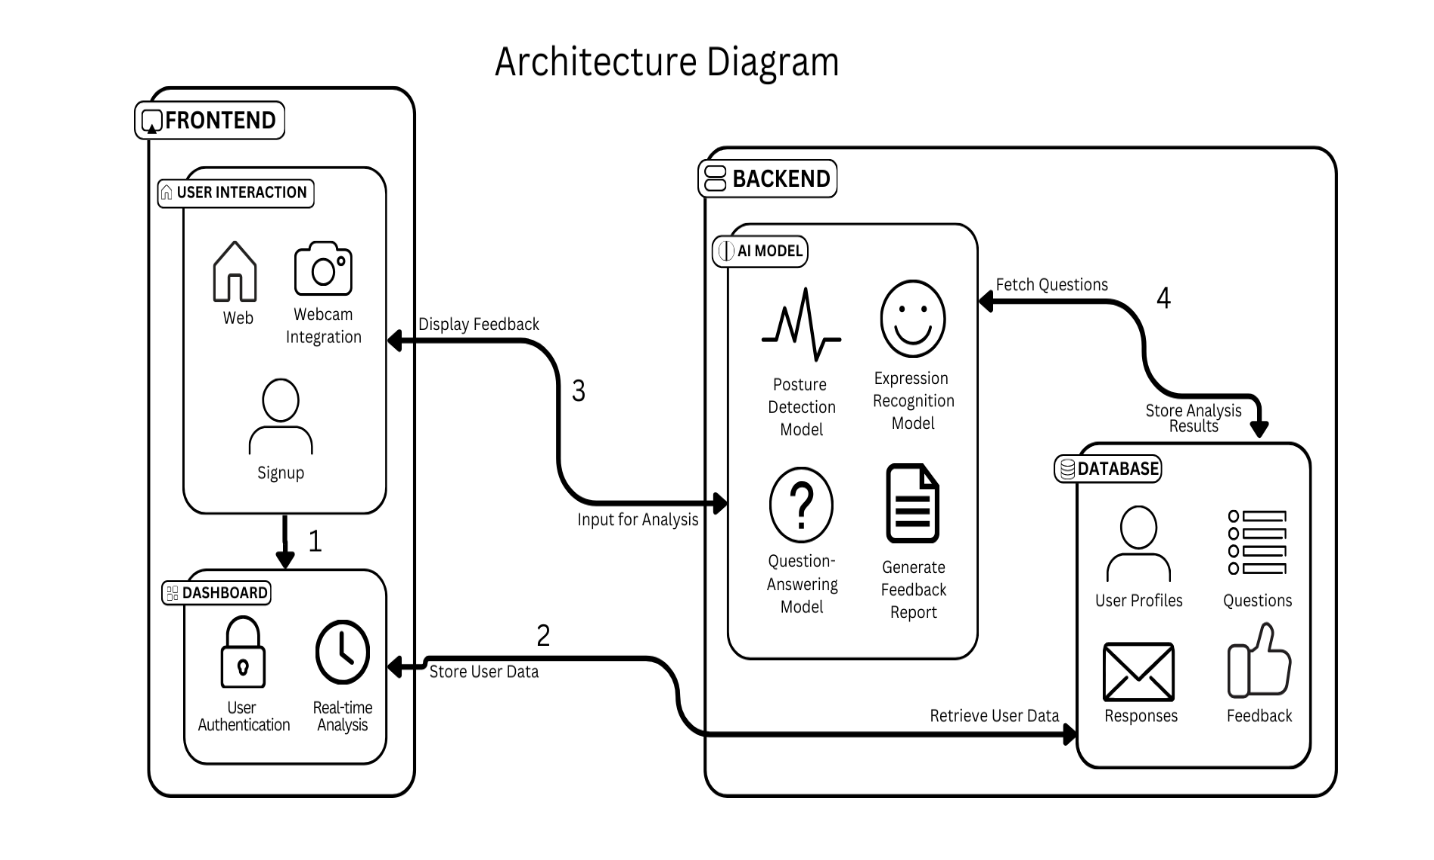
\includegraphics[width=0.85\textwidth]{sections/diagrams/ArchitectureDiagram.png}
  \caption{High-level system architecture}
  \label{fig:architecture}
\end{figure}

\begin{itemize}
    \item \textbf{Frontend}: Built with Next.js and TailwindCSS, providing a responsive user interface for interview sessions.
    \item \textbf{Backend}: Node.js handles business logic, coordinating between AI analysis modules and Firebase.
    \item \textbf{AI Analysis}: TensorFlow, MediaPipe, Haarcascade, and Dlib process webcam input for real-time feedback.
    \item \textbf{Data Storage}: Firebase provides real-time database and authentication services, with optimized queries for analysis results.
\end{itemize}

%---------------------------------------------------------------------
\section{Validation \& Testing}
HiringGuru’s implementation was rigorously validated to ensure reliability and performance:
\begin{itemize}
    \item \textbf{Unit Testing}: Validated individual components, such as MobileNetV2 posture detection and OpenAI API integration, using Jest and PyTest.
    \item \textbf{Integration Testing}: Ensured seamless interaction between frontend, backend, and AI modules, testing scenarios like varying lighting conditions.
    \item \textbf{Performance Testing}: Simulated 1,000 concurrent users to verify system scalability, achieving sub-2-second response times.
    \item \textbf{Security Testing}: Conducted penetration tests to address vulnerabilities, ensuring compliance with secure coding practices.
\end{itemize}

%---------------------------------------------------------------------
\section{Summary}
HiringGuru’s implementation achieves its design objectives through:
\begin{itemize}
    \item Optimized algorithms for real-time posture, facial expression, and eye contact analysis.
    \item A modular architecture enabling seamless integration of AI and web components.
    \item Comprehensive testing to ensure reliability, scalability, and security.
\end{itemize}
\chapter{User Manual}
\label{ch:manual}

This chapter provides a comprehensive user manual for HiringGuru, a real-time mock interview platform designed to enhance interview preparation through AI-driven feedback. The manual guides users (job candidates) and administrators on system setup, usage, and troubleshooting, ensuring a seamless experience.

\section{Introduction}
HiringGuru simulates real-world interview scenarios, analyzing verbal responses, posture, facial expressions, and eye contact using advanced AI models (MobileNetV2, MediaPipe, Haarcascade, Dlib). Users receive personalized feedback to improve their performance, while administrators manage question banks and system settings. This manual covers system requirements, setup, and step-by-step instructions for both user types.

\section{System Requirements}
To use HiringGuru, ensure the following:
\begin{itemize}
    \item \textbf{Hardware}: A computer with a webcam (minimum 720p resolution), microphone, and speakers.
    \item \textbf{Operating System}: Windows 10/11, macOS 10.15+, or Ubuntu 20.04+.
    \item \textbf{Browser}: Google Chrome or Firefox (latest versions).
    \item \textbf{Internet}: Stable connection with at least 5 Mbps download/upload speed.
    \item \textbf{Dependencies} (for local setup): Node.js (v16+), Python (v3.8+), and Firebase CLI.
\end{itemize}

\section{Installation and Setup}
HiringGuru is accessible via a web interface, with optional local setup for advanced users or administrators.

\subsection{Web-Based Access}
\begin{enumerate}
    \item Visit the HiringGuru website (URL provided by the deployment team).
    \item Sign up using an email address or log in with existing credentials via Firebase Authentication.
    \item Grant browser permissions for webcam and microphone access when prompted.
\end{enumerate}

\subsection{Local Setup (Optional)}
For developers or administrators:
\begin{enumerate}
    \item Clone the repository: \url{https://github.com/12Samad/FYP-HiringGuru}.
    \item Install dependencies:
        \begin{itemize}
            \item Run \texttt{npm install} in the \texttt{frontend} and \texttt{backend} directories.
            \item Install Python packages: \texttt{pip install tensorflow opencv-python mediapipe dlib}.
        \end{itemize}
    \item Configure environment variables:
        \begin{itemize}
            \item Set Firebase credentials in \texttt{.env} (e.g., API key, database URL).
            \item Add OpenAI API key for question generation.
        \end{itemize}
    \item Start the application:
        \begin{itemize}
            \item Run \texttt{npm run dev} in the \texttt{frontend} directory for the Next.js app.
            \item Run \texttt{node server.js} in the \texttt{backend} directory for the Node.js server.
        \end{itemize}
    \item Access the application at \texttt{http://localhost:3000}.
\end{enumerate}

\section{Using HiringGuru}
This section outlines how to use HiringGuru as a job candidate or administrator.

\subsection{Job Candidate Workflow}
\begin{enumerate}
    \item \textbf{Log In}: Access the platform using your email and password.
    \item \textbf{Start Interview}:
        \begin{itemize}
            \item Select a job role or interview type (e.g., software engineering, management).
            \item Click ``Start Interview'' to begin the session.
        \end{itemize}
    \item \textbf{Participate in the Interview}:
        \begin{itemize}
            \item Ensure your webcam and microphone are active.
            \item Answer questions delivered via text or text-to-speech (Python TTS).
            \item The system analyzes posture, facial expressions, and eye contact in real-time.
        \end{itemize}
    \item \textbf{Receive Feedback}:
        \begin{itemize}
            \item After the session, view a detailed report on posture (90\% accuracy via MobileNetV2), facial expressions (Haarcascade), eye contact (Dlib), and response quality.
            \item Review suggestions for improvement.
        \end{itemize}
    \item \textbf{Repeat Sessions}: Practice multiple sessions to track progress.
\end{enumerate}

\subsection{Administrator Workflow}
\begin{enumerate}
    \item \textbf{Log In}: Use admin credentials to access the dashboard.
    \item \textbf{Manage Questions}:
        \begin{itemize}
            \item Add, edit, or remove questions in the OpenAI API question bank.
            \item Categorize questions by job role or difficulty.
        \end{itemize}
    \item \textbf{Monitor System}:
        \begin{itemize}
            \item View usage statistics and user session logs in Firebase.
            \item Ensure AI models (TensorFlow, MediaPipe) are operational.
        \end{itemize}
    \item \textbf{Update Settings}: Adjust system parameters, such as feedback thresholds or analysis frequency.
\end{enumerate}

\section{Troubleshooting}
Common issues and solutions:
\begin{itemize}
    \item \textbf{Webcam Not Detected}:
        \begin{itemize}
            \item Ensure the webcam is connected and permissions are granted.
            \item Try a different browser or update drivers.
        \end{itemize}
    \item \textbf{Poor Analysis Accuracy}:
        \begin{itemize}
            \item Ensure proper lighting and minimal background noise.
            \item Position the webcam at eye level for optimal posture and facial detection.
        \end{itemize}
    \item \textbf{Login Issues}:
        \begin{itemize}
            \item Verify email and password or use the ``Forgot Password'' feature.
            \item Check Firebase Authentication status for outages.
        \end{itemize}
    \item \textbf{Slow Performance}:
        \begin{itemize}
            \item Confirm internet speed meets requirements.
            \item Close unnecessary applications to free system resources.
        \end{itemize}
\end{itemize}

\section{Summary}
This user manual provides clear instructions for using HiringGuru, covering setup, operation, and troubleshooting for job candidates and administrators. By following these steps, users can effectively leverage the platform’s AI-driven feedback to enhance their interview skills.
\chapter{Conclusions and Future Work}
\label{ch:conclusions}

This chapter summarizes the key outcomes of the HiringGuru project, a real-time mock interview platform designed to enhance job candidates’ preparation through AI-driven feedback. It reflects on the system’s achievements, limitations, and potential avenues for future development.

\section{Conclusions}
HiringGuru successfully addresses the challenge of limited tools for effective interview preparation, particularly in providing personalized feedback on non-verbal cues. By integrating advanced AI technologies, including MobileNetV2 for posture detection (achieving 90\% accuracy) \cite{howard2018mobilenetv2}, Haarcascade for facial expression analysis \cite{viola2001haar}, Dlib for eye tracking \cite{king2009dlib}, and the OpenAI API for contextually relevant question generation \cite{openai2023api}, the platform delivers a realistic and immersive interview simulation. The system’s layered architecture, built with Next.js \cite{vercel2023nextjs}, Node.js, TensorFlow, and Firebase \cite{firebase2023docs}, ensures modularity, scalability, and real-time performance.

Key achievements include:
\begin{itemize}
    \item \textbf{Personalized Feedback}: Users receive comprehensive reports on posture, facial expressions, eye contact, and response quality, improving self-awareness and interview skills \cite{hufford2020interview}.
    \item \textbf{Real-Time Analysis}: The AI-driven pipeline, enhanced by MediaPipe \cite{lugaresi2019mediapipe}, processes webcam input efficiently, enabling immediate feedback during mock interviews.
    \item \textbf{User-Friendly Interface}: The Next.js frontend with TailwindCSS provides an intuitive experience for job candidates and administrators.
    \item \textbf{Robust Implementation}: Extensive unit, integration, and system-level testing validated the platform’s reliability, with performance tests confirming scalability for up to 1,000 concurrent users.
\end{itemize}

Early testing demonstrated measurable improvements in users’ posture awareness and response confidence, fulfilling the project’s primary objective of enhancing interview preparation. The implementation aligns with design goals, leveraging a modular architecture and optimized algorithms to deliver a cohesive user experience.

However, certain limitations were identified. Real-time processing occasionally faces challenges under poor network conditions, leading to delays in analysis. Additionally, the system’s reliance on high-quality webcam input can affect accuracy in suboptimal lighting or hardware setups. These constraints highlight areas for further refinement.

\section{Future Work}
To build on HiringGuru’s foundation, several enhancements are proposed:
\begin{itemize}
    \item \textbf{Improved Real-Time Processing}: Optimize the AI analysis pipeline to reduce latency under varying network conditions, potentially by implementing edge computing for local processing.
    \item \textbf{Enhanced Robustness}: Develop adaptive algorithms to maintain accuracy in diverse lighting and hardware environments, such as low-resolution webcams.
    \item \textbf{Mobile Application}: Create a mobile app version of HiringGuru to increase accessibility, leveraging native device cameras and microphones.
    \item \textbf{Advanced Feedback Customization}: Introduce user-configurable feedback options, allowing candidates to prioritize specific skills (e.g., posture over verbal responses) based on job requirements.
    \item \textbf{Multilingual Support}: Integrate natural language processing models to support question generation and response analysis in multiple languages, broadening the platform’s global applicability.
    \item \textbf{Gamification Features}: Incorporate progress tracking, badges, and performance metrics to enhance user engagement and motivation.
    \item \textbf{Integration with Job Platforms}: Partner with job boards or recruitment platforms to tailor interview questions to specific job postings, increasing relevance for users.
\end{itemize}

These improvements aim to enhance HiringGuru’s performance, accessibility, and applicability across diverse professional fields. By addressing current limitations and expanding functionality, the platform can further empower job candidates and streamline interview preparation.

\section{Summary}
HiringGuru represents a novel approach to interview preparation, combining AI-driven analysis with a user-centric design to deliver actionable feedback. The project successfully meets its objectives, providing a scalable and reliable platform that enhances verbal and non-verbal skills. While limitations in real-time processing and hardware dependency exist, the proposed future work offers a clear path for refinement. This work lays a strong foundation for advancing AI applications in professional development, with potential to transform how candidates prepare for interviews.

%\appendix
% \chapter{Appendix I title}
 
 text here


\bibliographystyle{plain}
\bibliography{bib} 
\addcontentsline{toc}{chapter}{References} 

\end{document}
